\documentclass[11pt,letterpaper]{article}

\usepackage{showlabels}
\usepackage{fullpage}
\usepackage{pslatex}
%\usepackage{latexsym}
\usepackage[english]{babel}
\usepackage[utf8]{inputenc}
\usepackage{amsmath}
\usepackage{bm}
\usepackage{graphicx}
\usepackage{tikz}
\usepackage{xcolor}
\usepackage{url}
%\usepackage[colorinlistoftodos]{todonotes}
\usepackage{rotating}
\usepackage{natbib}
\usepackage{amssymb}

\usepackage{tikz-dependency}
\usepackage{longtable}


\newcommand{\R}[0]{\mathbb{R}}
\newcommand{\E}[0]{\mathbb{E}}
\newcommand{\Ff}[0]{\mathcal{F}}

\usepackage{multirow}

\newcommand{\soft}[1]{}
\newcommand{\nopreview}[1]{}
\newcommand\comment[1]{{\color{red}#1}}
\newcommand\mhahn[1]{{\color{red}(#1)}}

\usepackage{amsthm}

\newcommand{\thetad}[0]{{\theta_d}}
\newcommand{\thetal}[0]{{\theta_{LM}}}

\newcounter{theorem}
\newtheorem{proposition}[theorem]{Proposition}
\newtheorem{thm}[theorem]{Theorem}
\newtheorem{corollary}[theorem]{Corollary}
\newtheorem{question}[theorem]{Question}
\newtheorem{example}[theorem]{Example}
\newtheorem{lemma}[theorem]{Lemma}


\frenchspacing
%\def\baselinestretch{0.975}

%\emnlpfinalcopy
%\def\emnlppaperid{496}

\title{Crosslinguistic Word Orders Enable an Efficient Tradeoff between Memory and Surprisal}
\author{Michael Hahn, Judith Degen, Richard Futrell}
\date{2018}

\begin{document}

\maketitle


\begin{table}
\begin{longtable}{ccccccccccccccclll}
Afrikaans & Amharic & Arabic & Armenian & Bambara & Basque & Breton & Bulgarian & Buryat
 \\ 
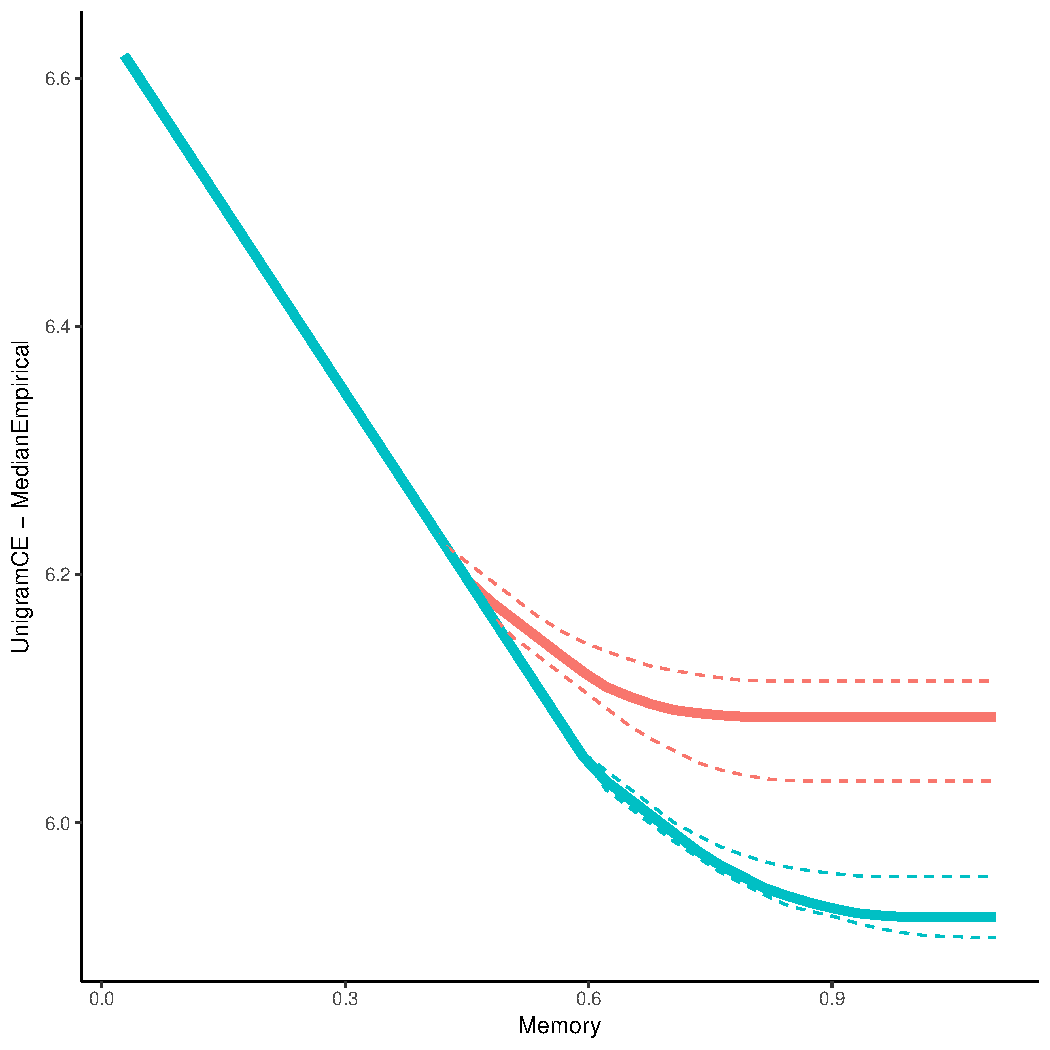
\includegraphics[width=0.1\textwidth]{neural/figures/Afrikaans-listener-surprisal-memory-MEDIANS_onlyWordForms_boundedVocab_REAL.pdf} & 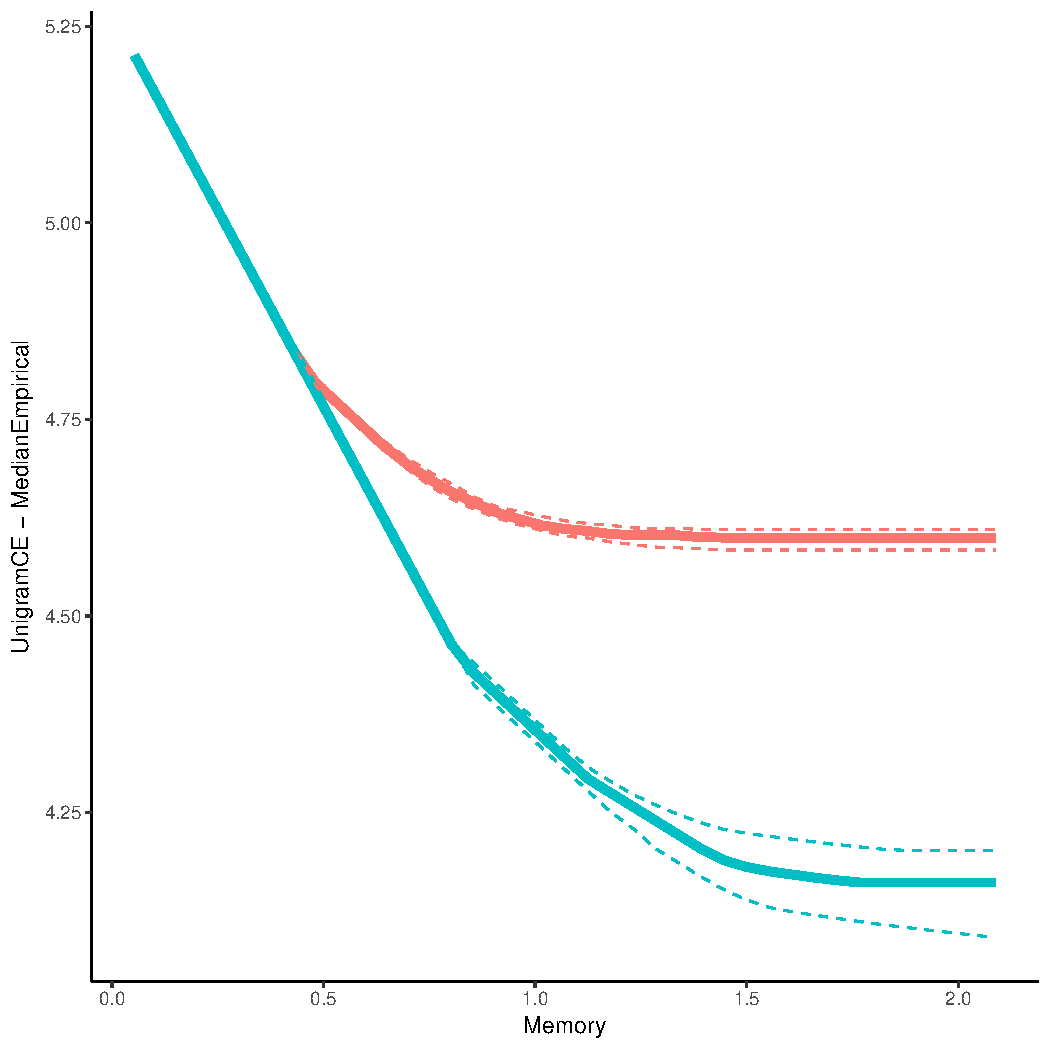
\includegraphics[width=0.1\textwidth]{neural/figures/Amharic-Adap-listener-surprisal-memory-MEDIANS_onlyWordForms_boundedVocab_REAL.pdf} & 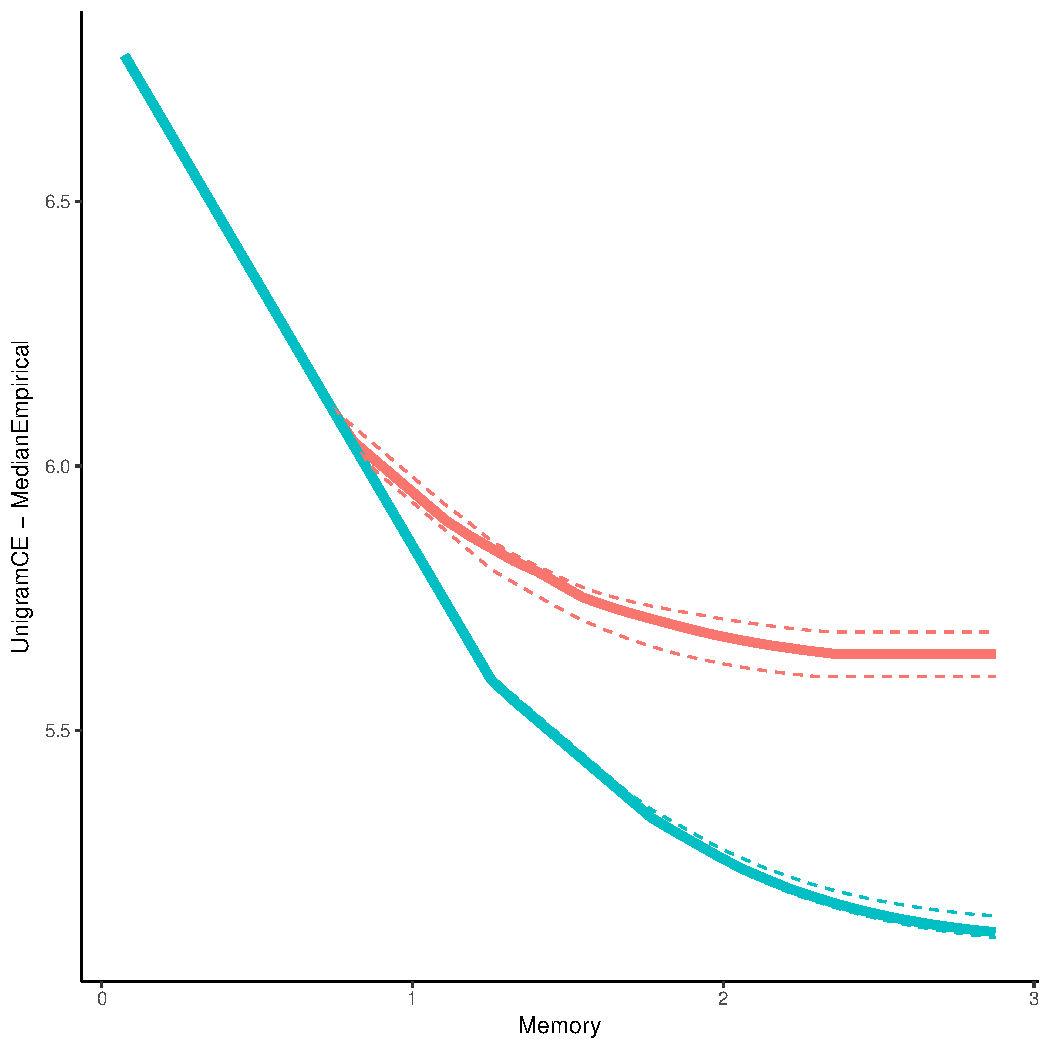
\includegraphics[width=0.1\textwidth]{neural/figures/Arabic-listener-surprisal-memory-MEDIANS_onlyWordForms_boundedVocab_REAL.pdf} & 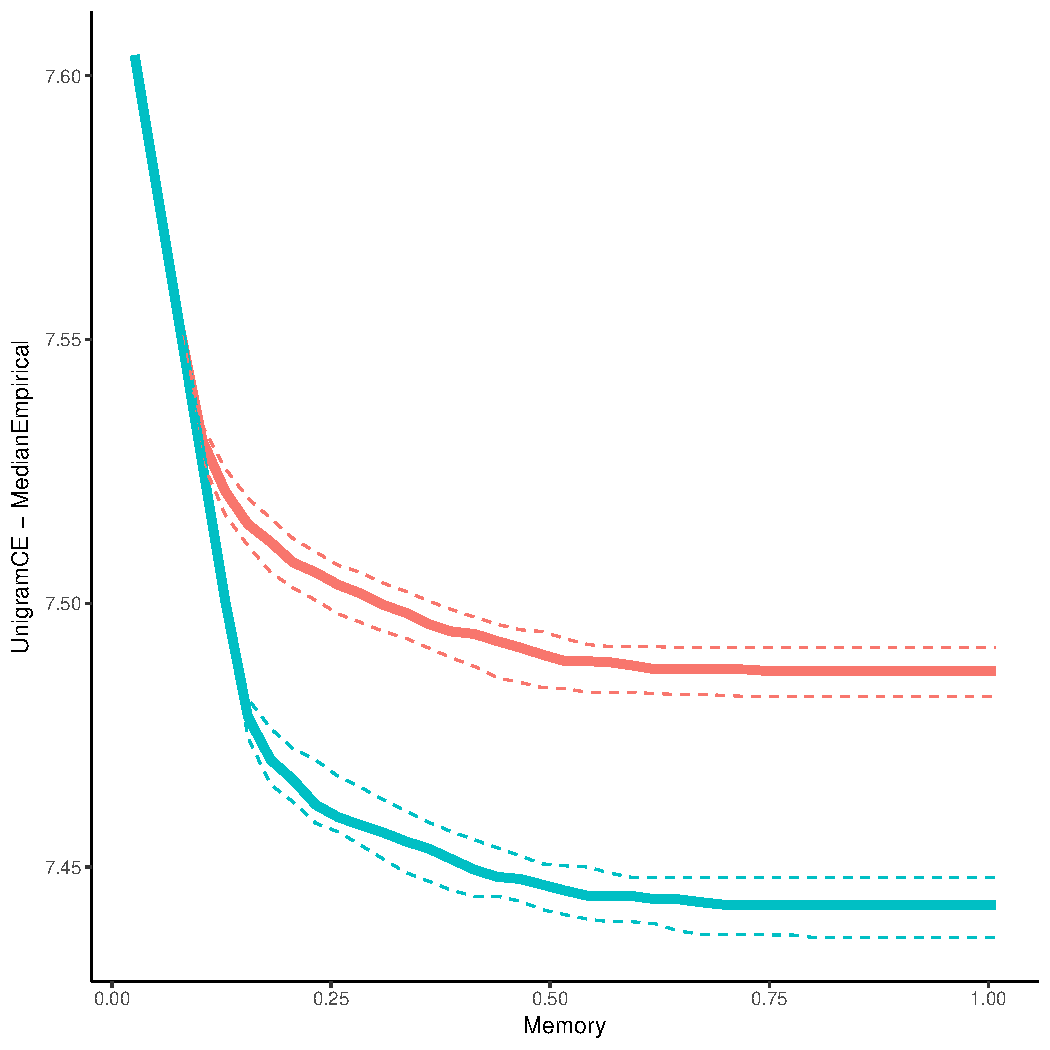
\includegraphics[width=0.1\textwidth]{neural/figures/Armenian-Adap-listener-surprisal-memory-MEDIANS_onlyWordForms_boundedVocab_REAL.pdf} & 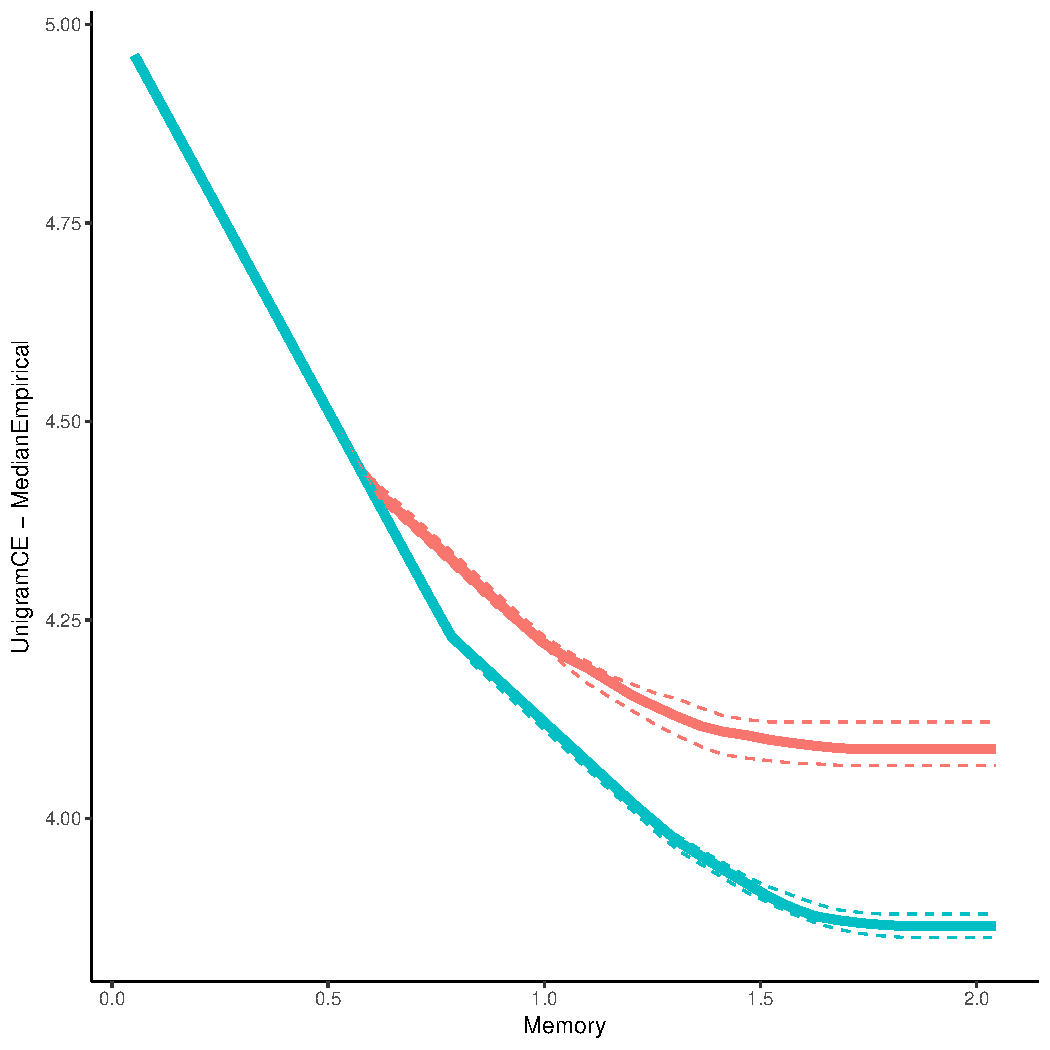
\includegraphics[width=0.1\textwidth]{neural/figures/Bambara-Adap-listener-surprisal-memory-MEDIANS_onlyWordForms_boundedVocab_REAL.pdf} & 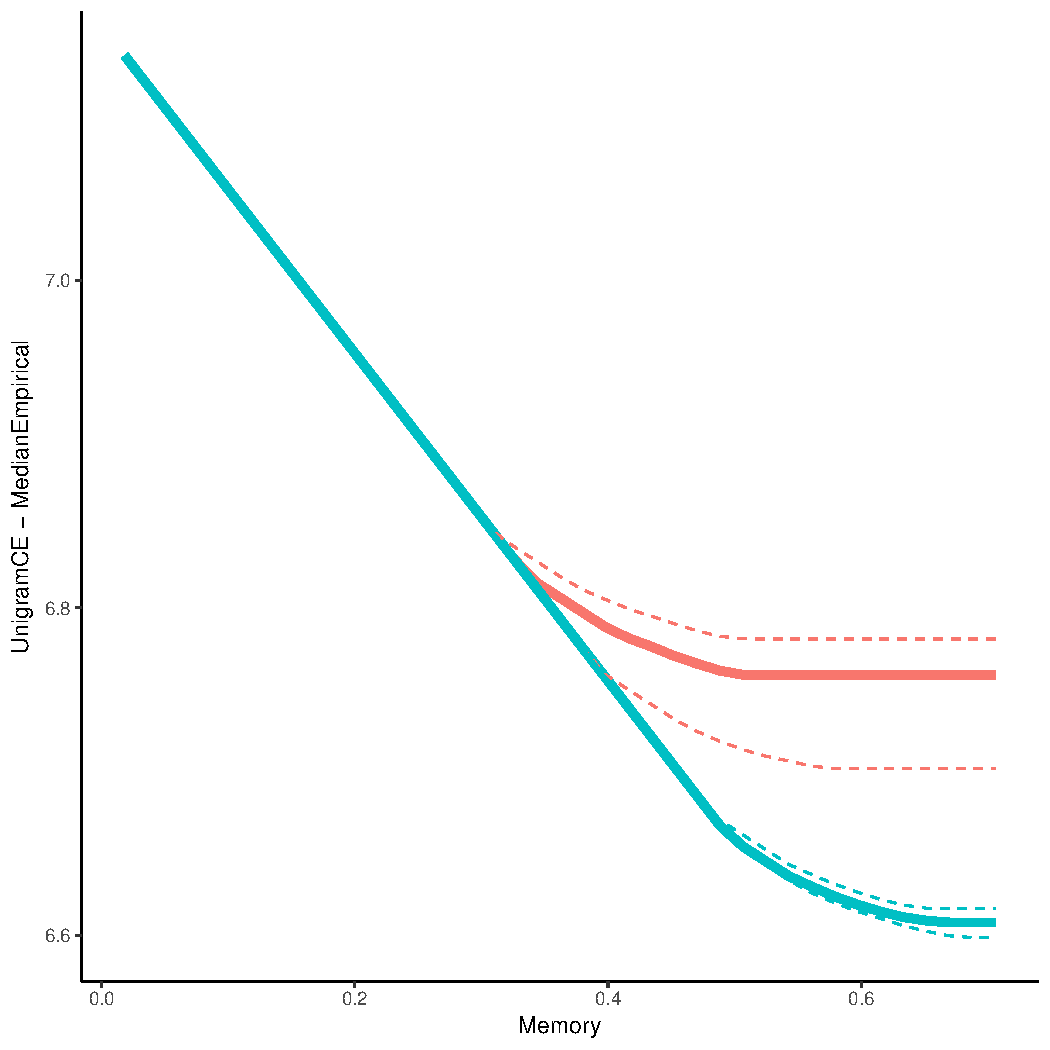
\includegraphics[width=0.1\textwidth]{neural/figures/Basque-listener-surprisal-memory-MEDIANS_onlyWordForms_boundedVocab_REAL.pdf} & 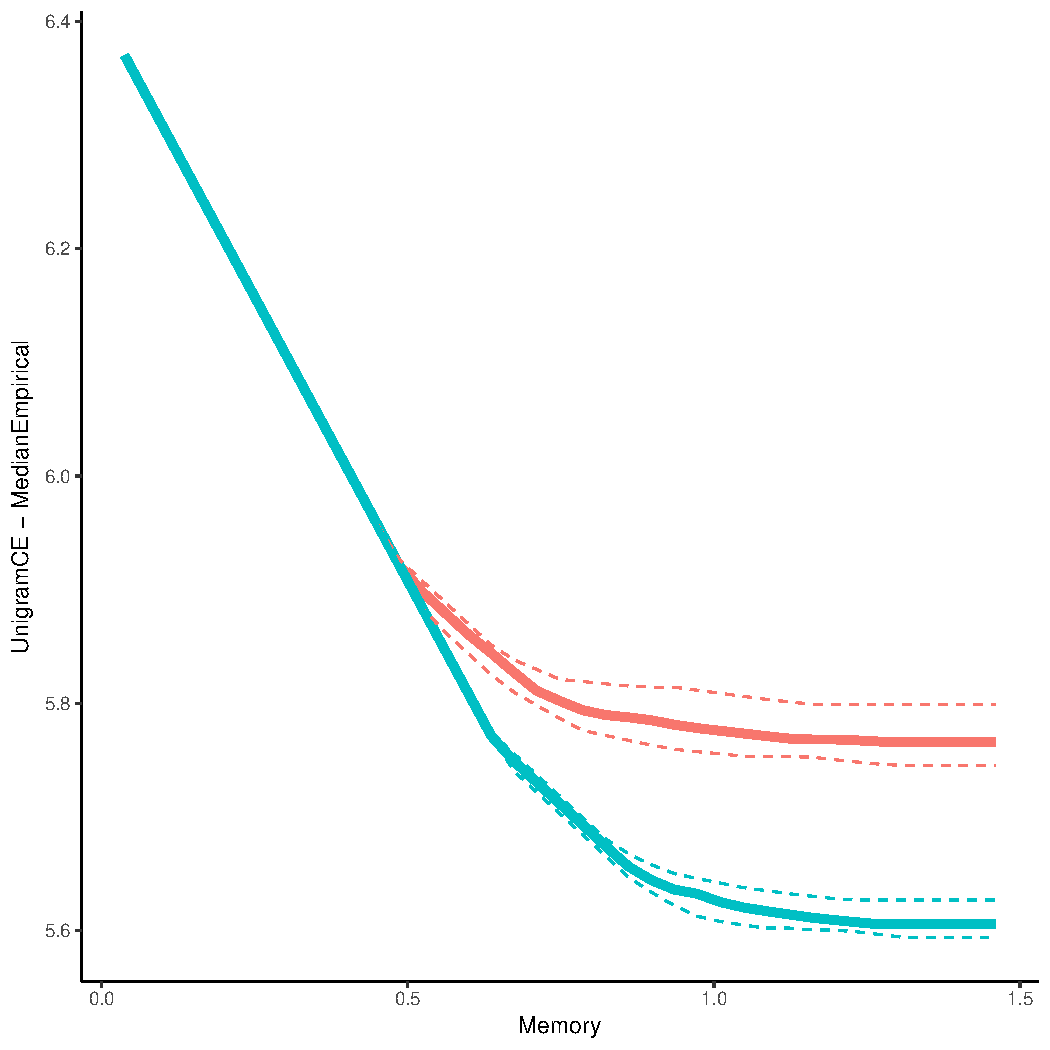
\includegraphics[width=0.1\textwidth]{neural/figures/Breton-Adap-listener-surprisal-memory-MEDIANS_onlyWordForms_boundedVocab_REAL.pdf} & 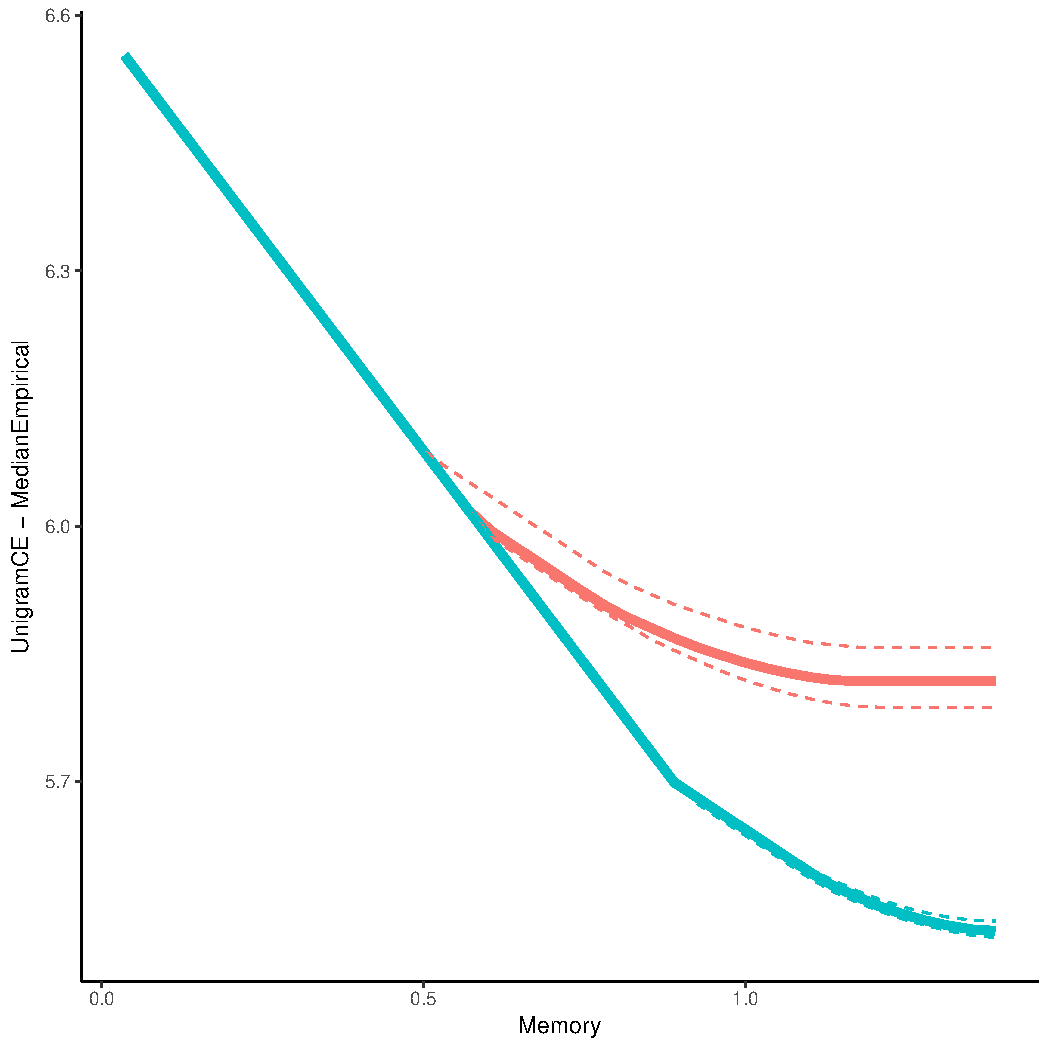
\includegraphics[width=0.1\textwidth]{neural/figures/Bulgarian-listener-surprisal-memory-MEDIANS_onlyWordForms_boundedVocab_REAL.pdf} & 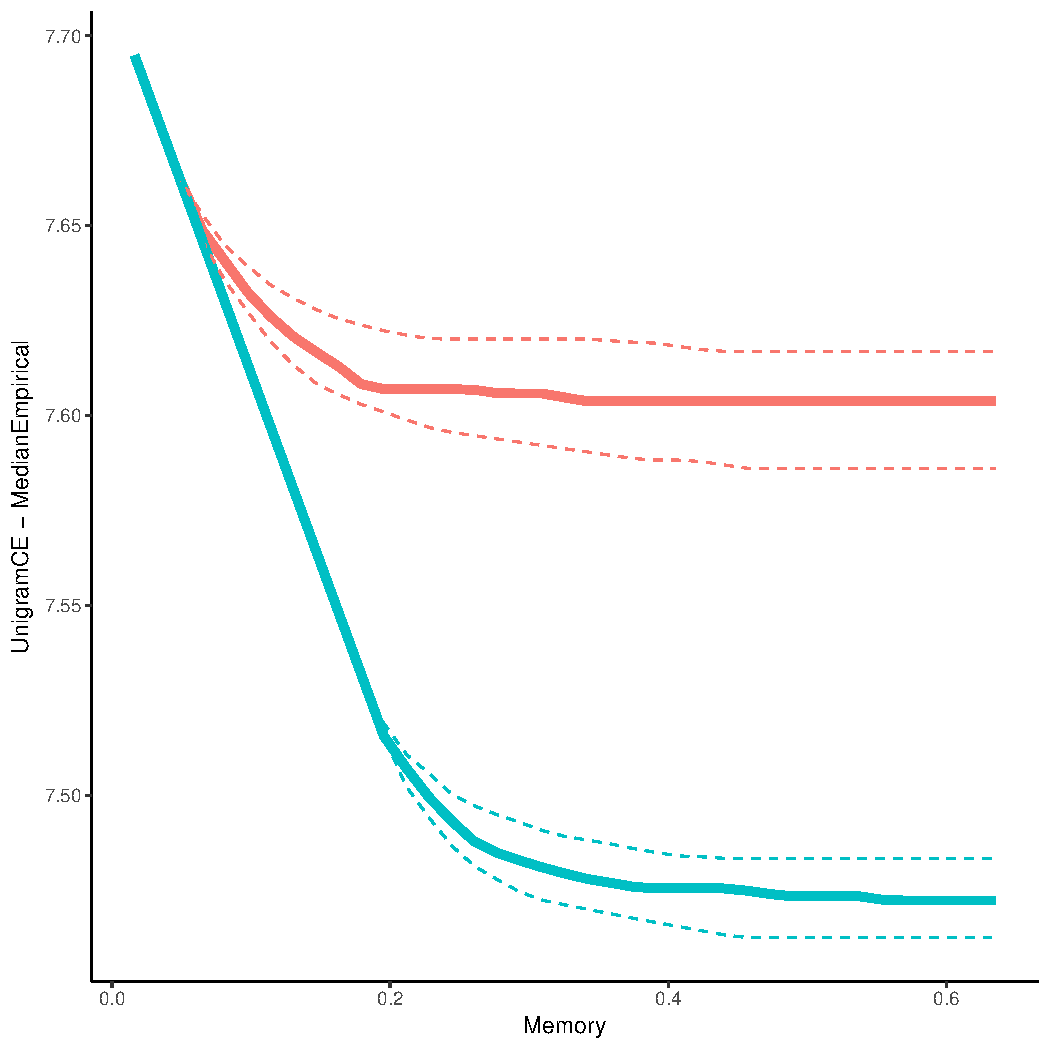
\includegraphics[width=0.1\textwidth]{neural/figures/Buryat-Adap-listener-surprisal-memory-MEDIANS_onlyWordForms_boundedVocab_REAL.pdf}
 \\ 
Cantonese & Catalan & Chinese & Croatian & Czech & Danish & Dutch & English & Erzya
 \\ 
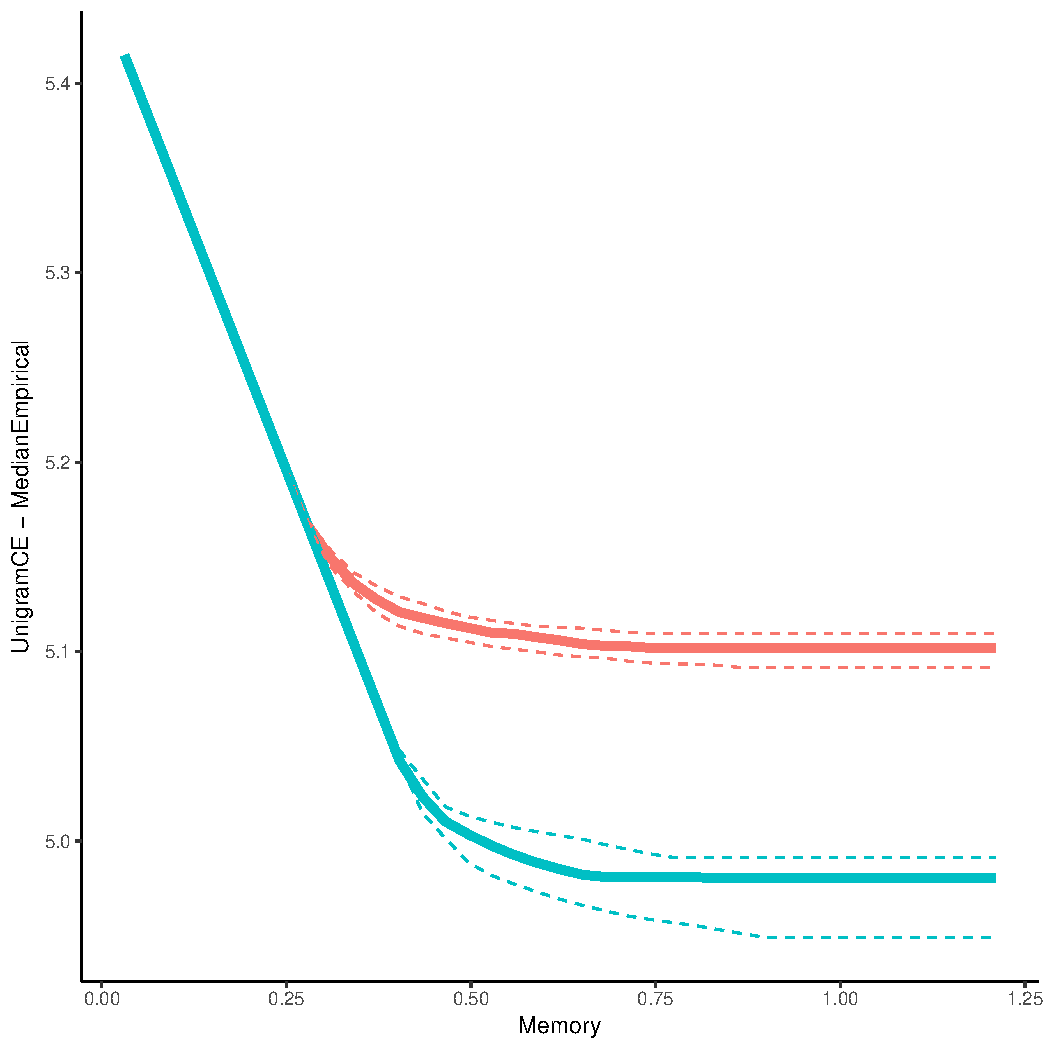
\includegraphics[width=0.1\textwidth]{neural/figures/Cantonese-Adap-listener-surprisal-memory-MEDIANS_onlyWordForms_boundedVocab_REAL.pdf} & 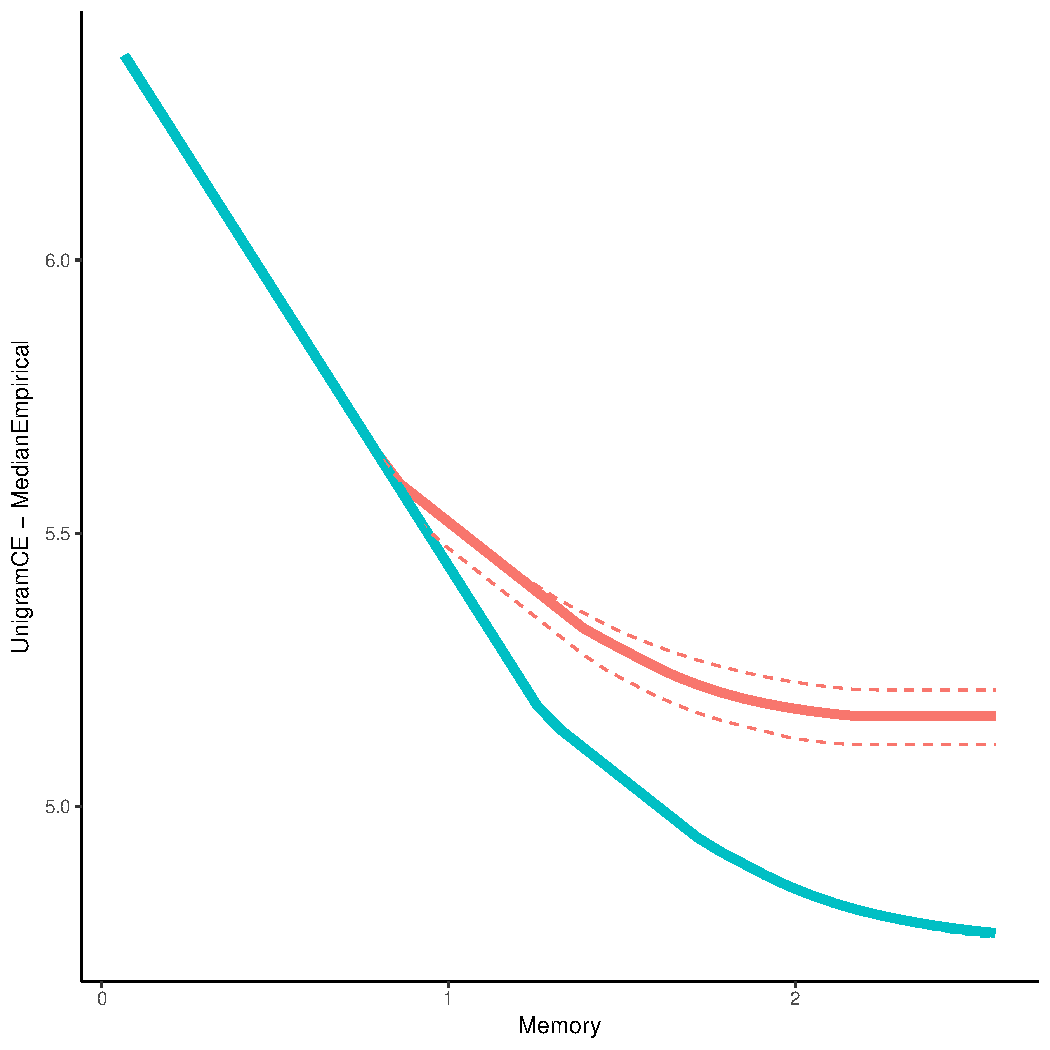
\includegraphics[width=0.1\textwidth]{neural/figures/Catalan-listener-surprisal-memory-MEDIANS_onlyWordForms_boundedVocab_REAL.pdf} & 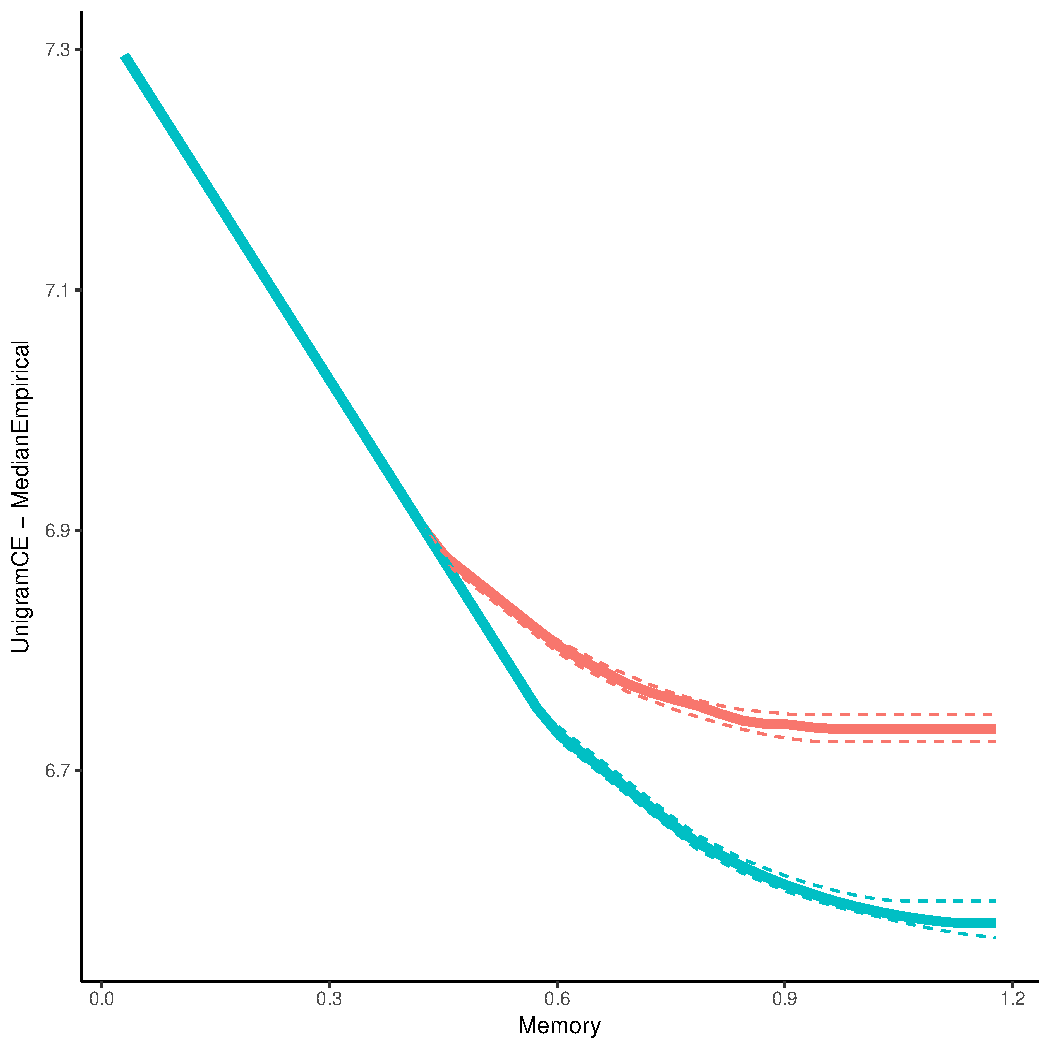
\includegraphics[width=0.1\textwidth]{neural/figures/Chinese-listener-surprisal-memory-MEDIANS_onlyWordForms_boundedVocab_REAL.pdf} & 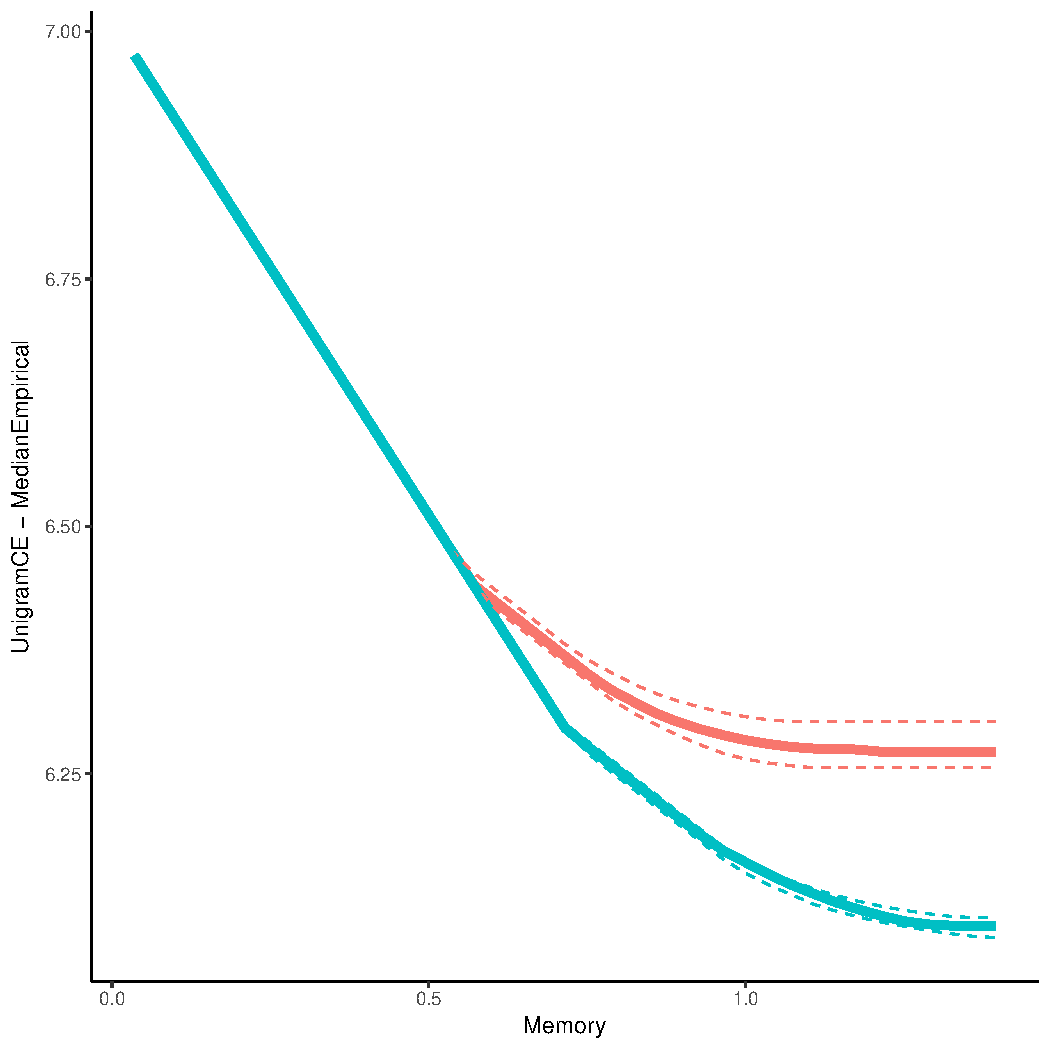
\includegraphics[width=0.1\textwidth]{neural/figures/Croatian-listener-surprisal-memory-MEDIANS_onlyWordForms_boundedVocab_REAL.pdf} & 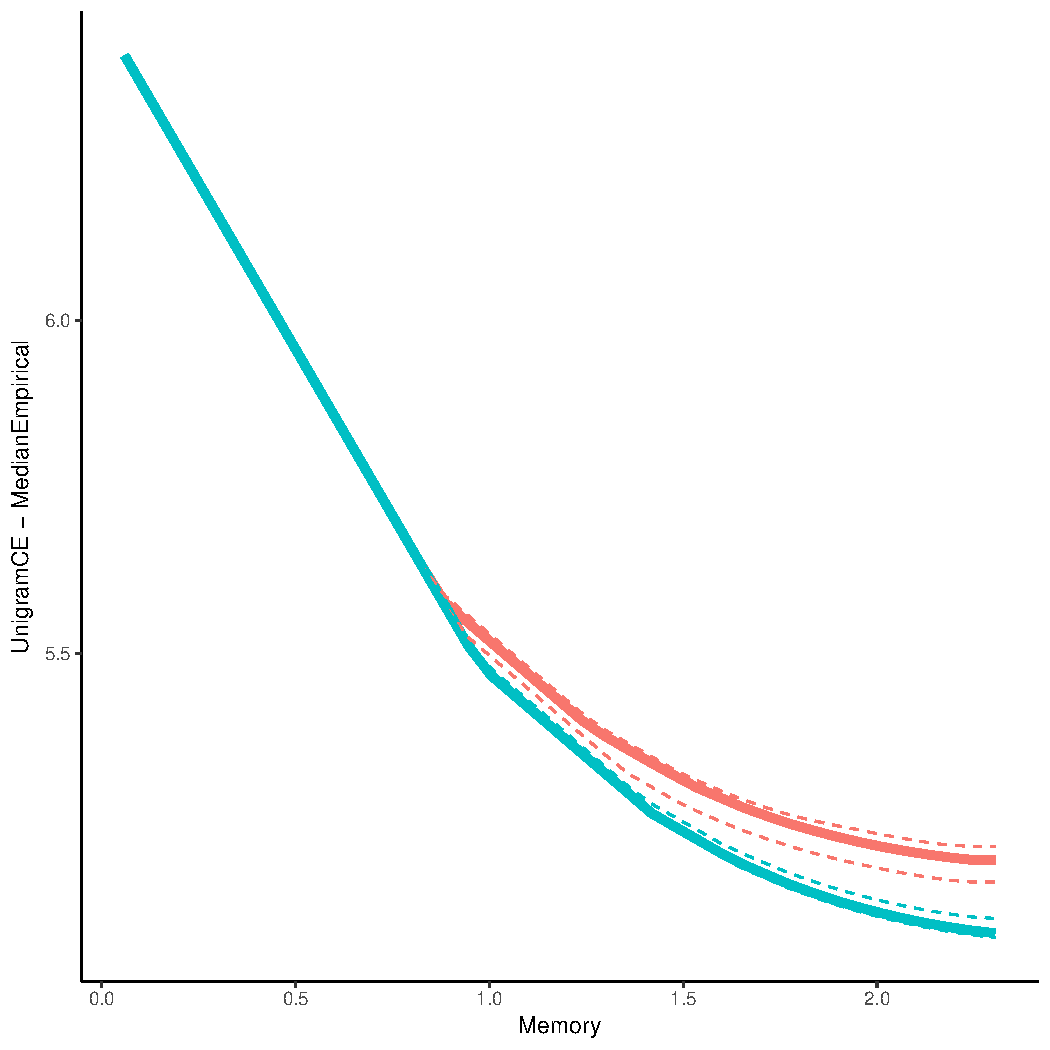
\includegraphics[width=0.1\textwidth]{neural/figures/Czech-listener-surprisal-memory-MEDIANS_onlyWordForms_boundedVocab_REAL.pdf} & 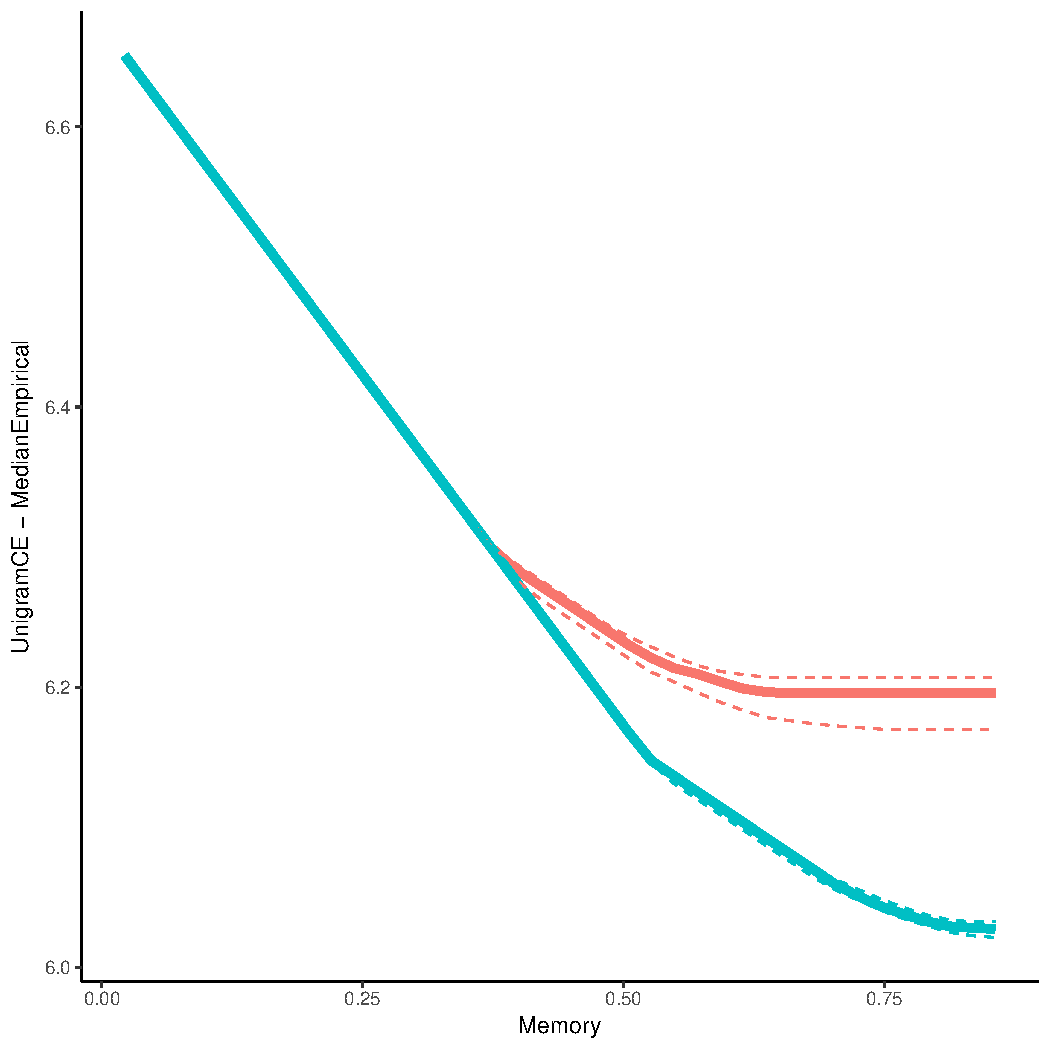
\includegraphics[width=0.1\textwidth]{neural/figures/Danish-listener-surprisal-memory-MEDIANS_onlyWordForms_boundedVocab_REAL.pdf} & 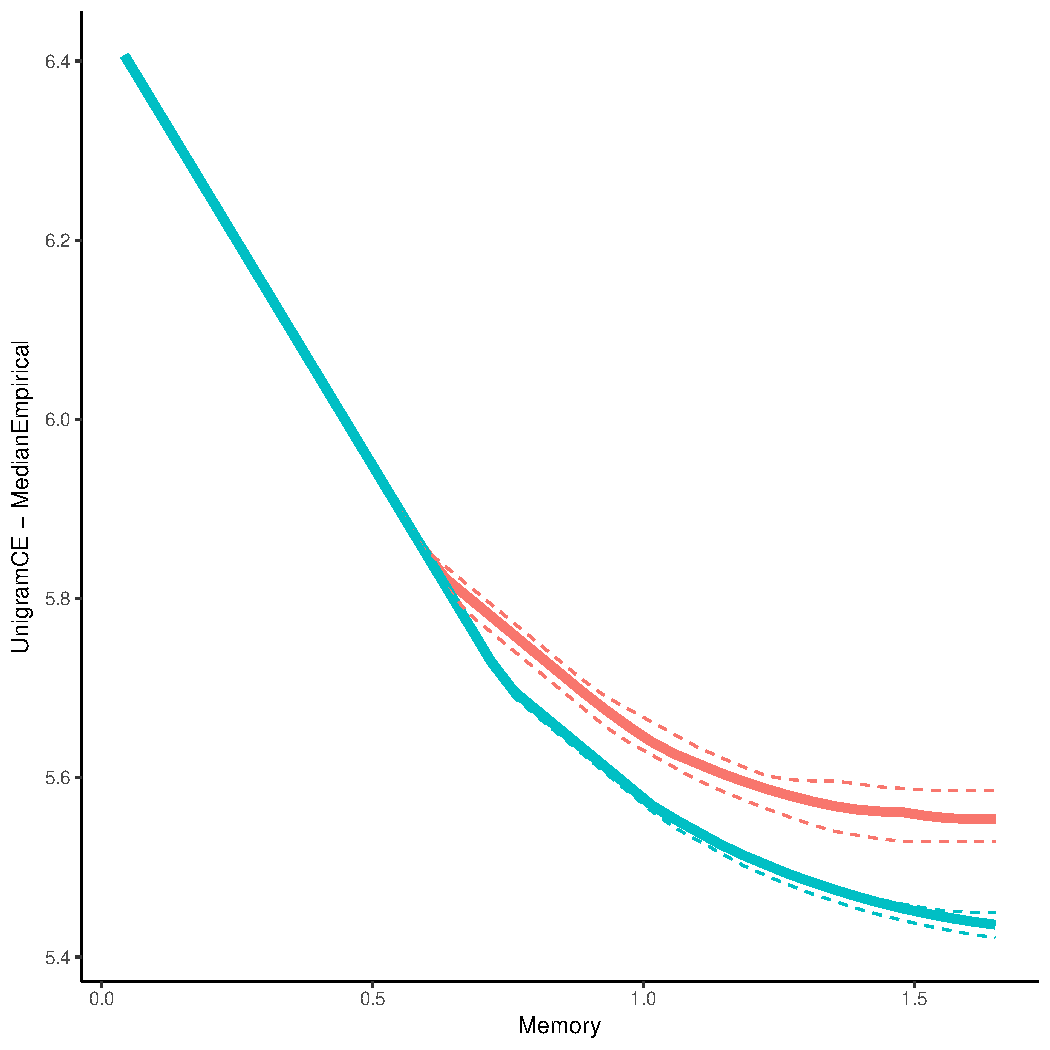
\includegraphics[width=0.1\textwidth]{neural/figures/Dutch-listener-surprisal-memory-MEDIANS_onlyWordForms_boundedVocab_REAL.pdf} & 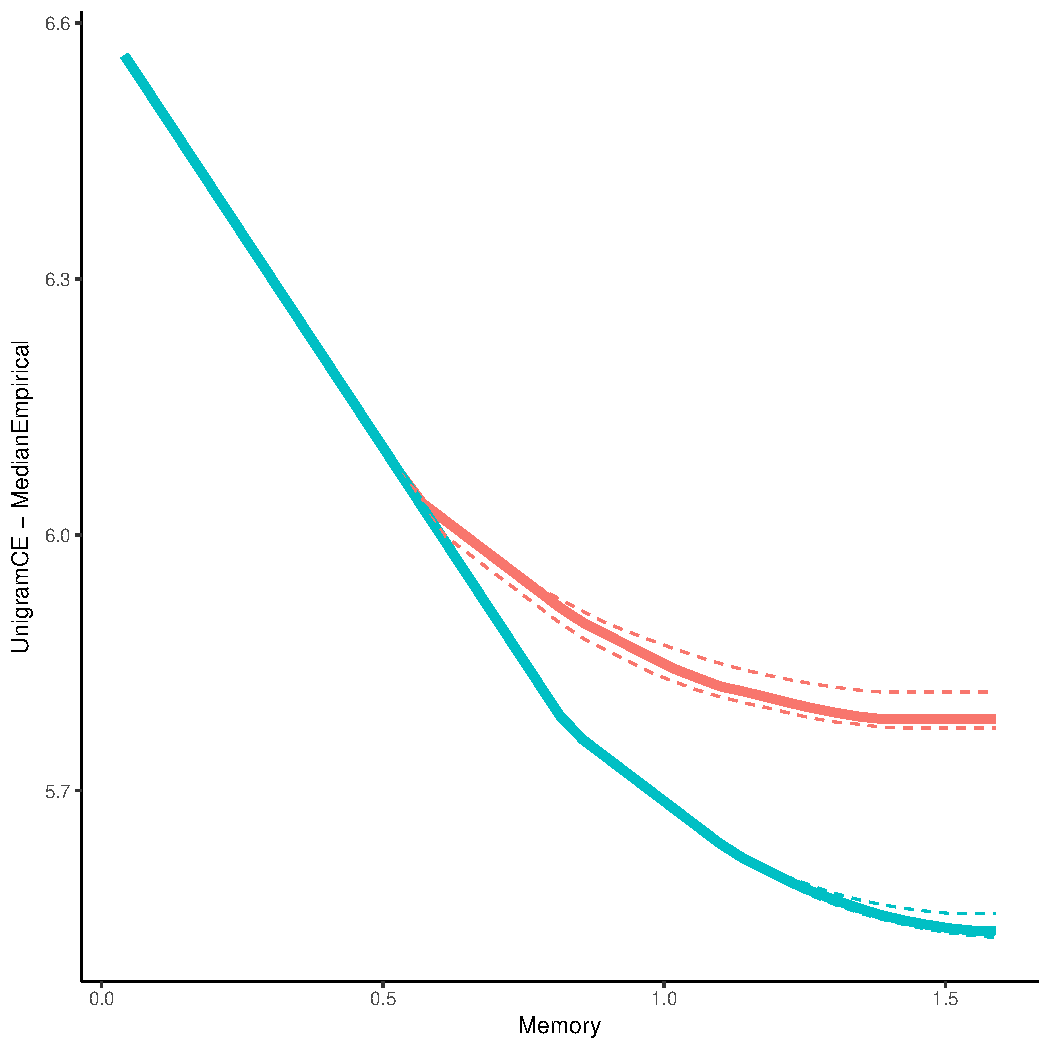
\includegraphics[width=0.1\textwidth]{neural/figures/English-listener-surprisal-memory-MEDIANS_onlyWordForms_boundedVocab_REAL.pdf} & 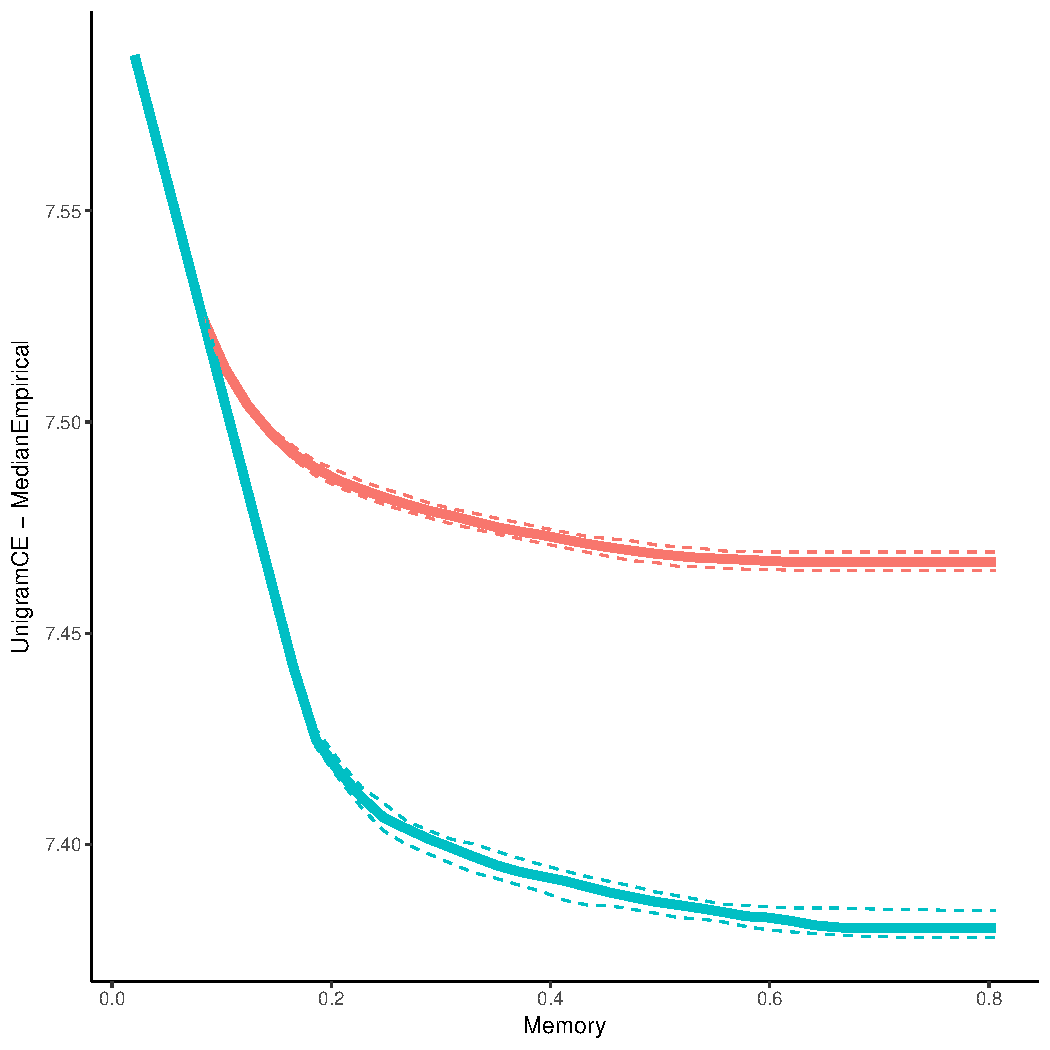
\includegraphics[width=0.1\textwidth]{neural/figures/Erzya-Adap-listener-surprisal-memory-MEDIANS_onlyWordForms_boundedVocab_REAL.pdf}
 \\ 
Estonian & Faroese & Finnish & French & German & Greek & Hebrew & Hindi & Hungarian
 \\ 
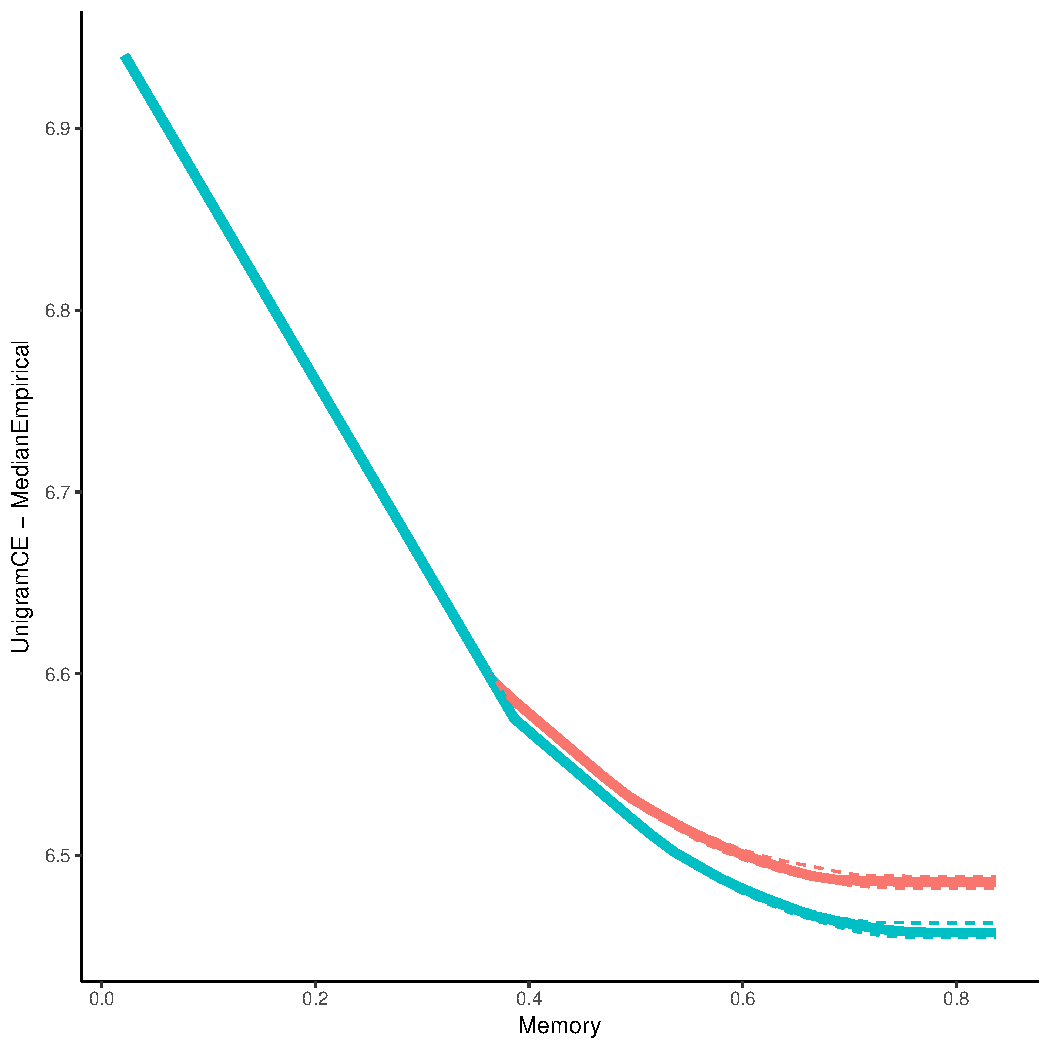
\includegraphics[width=0.1\textwidth]{neural/figures/Estonian-listener-surprisal-memory-MEDIANS_onlyWordForms_boundedVocab_REAL.pdf} & 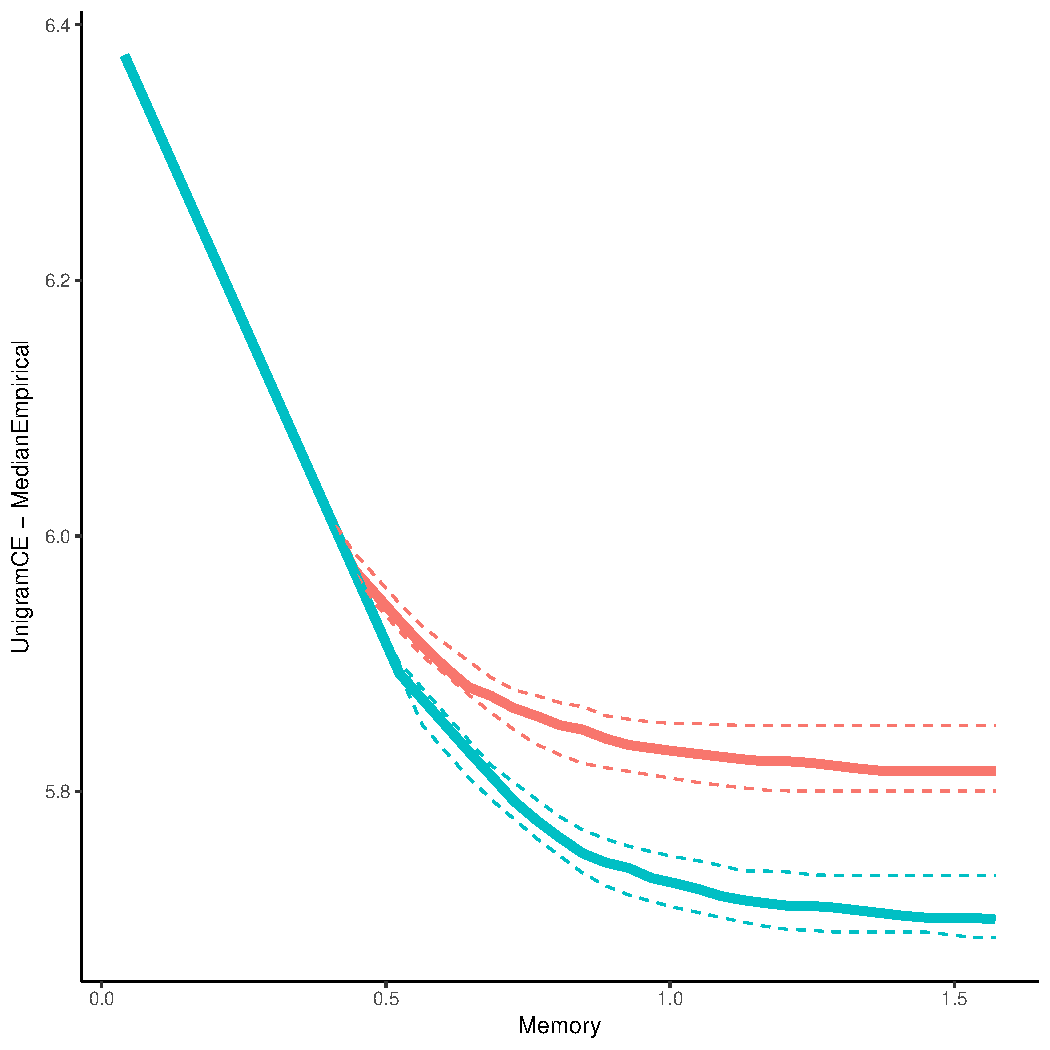
\includegraphics[width=0.1\textwidth]{neural/figures/Faroese-Adap-listener-surprisal-memory-MEDIANS_onlyWordForms_boundedVocab_REAL.pdf} & 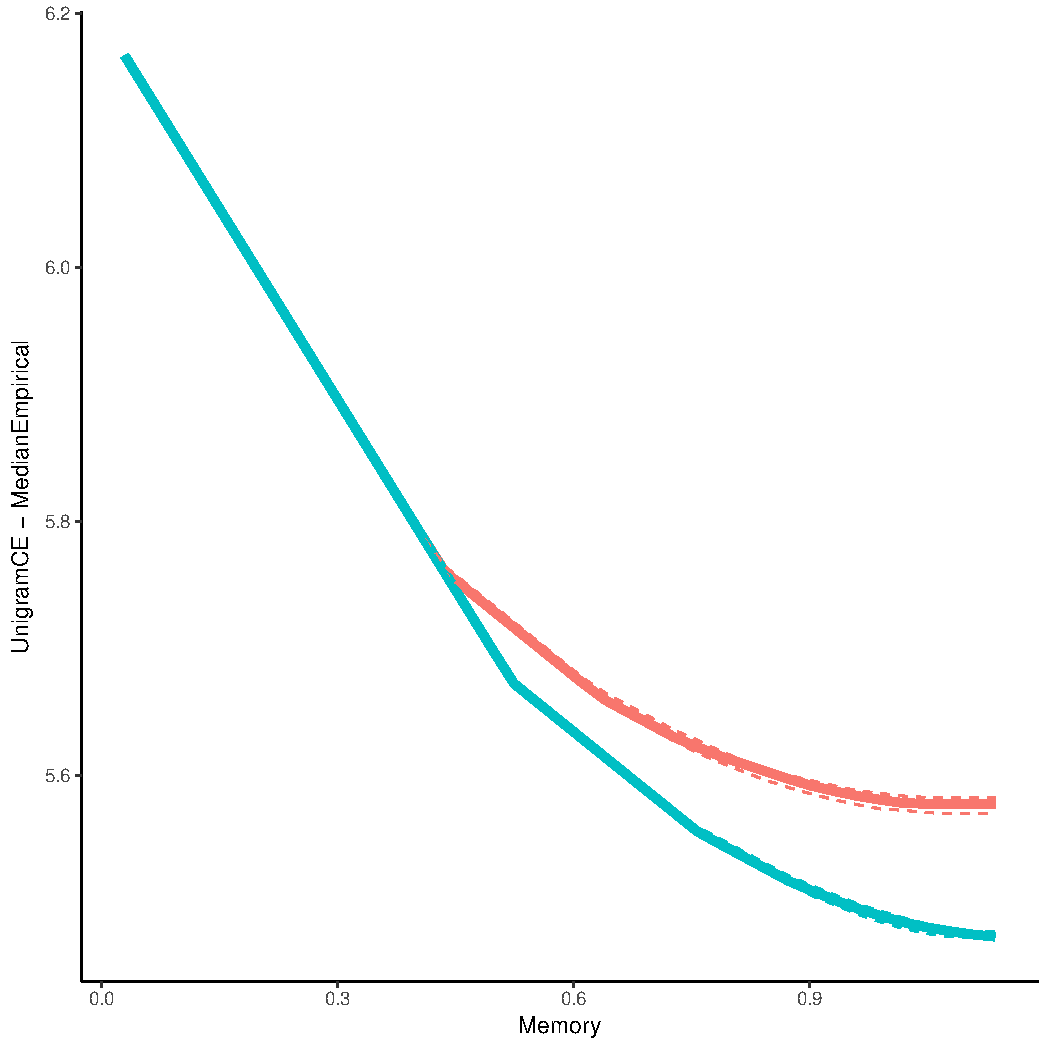
\includegraphics[width=0.1\textwidth]{neural/figures/Finnish-listener-surprisal-memory-MEDIANS_onlyWordForms_boundedVocab_REAL.pdf} & 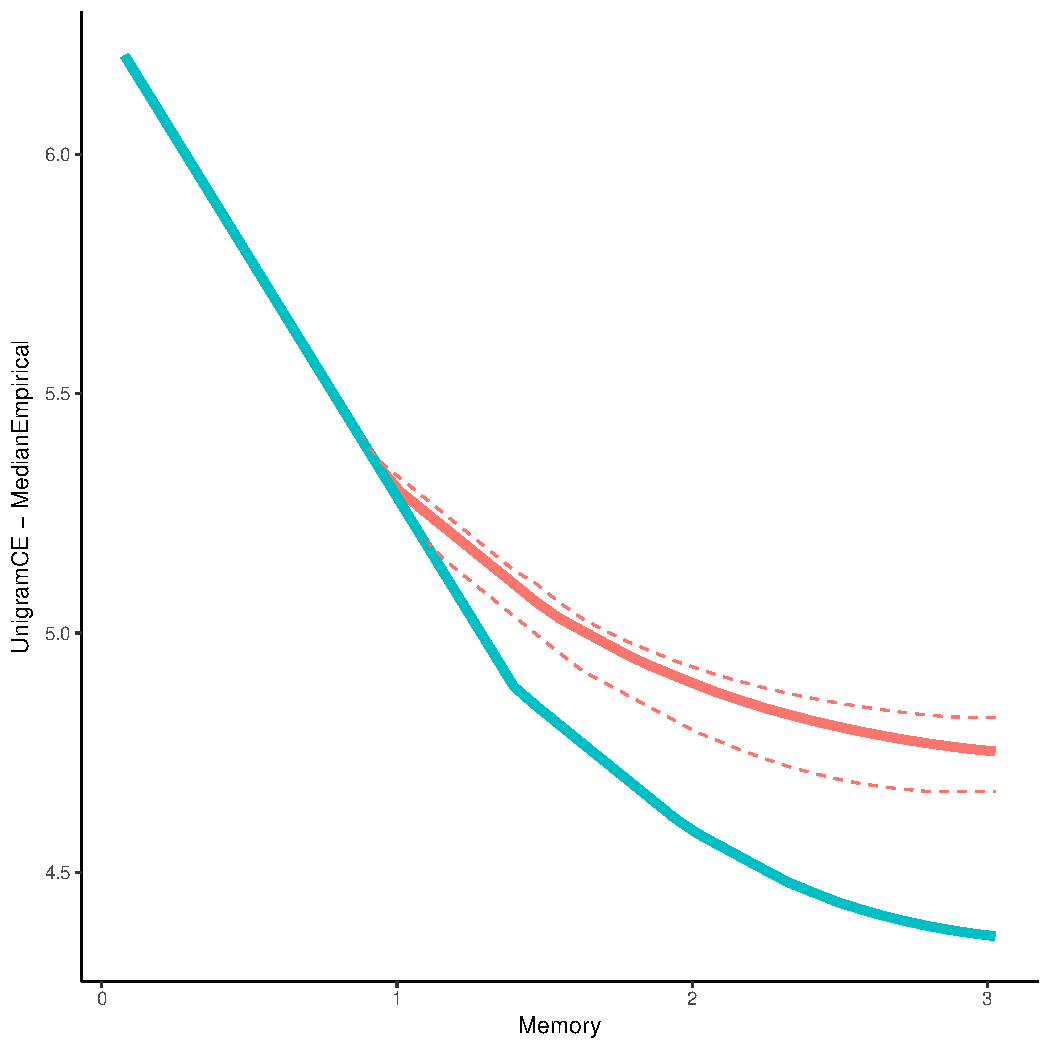
\includegraphics[width=0.1\textwidth]{neural/figures/French-listener-surprisal-memory-MEDIANS_onlyWordForms_boundedVocab_REAL.pdf} & 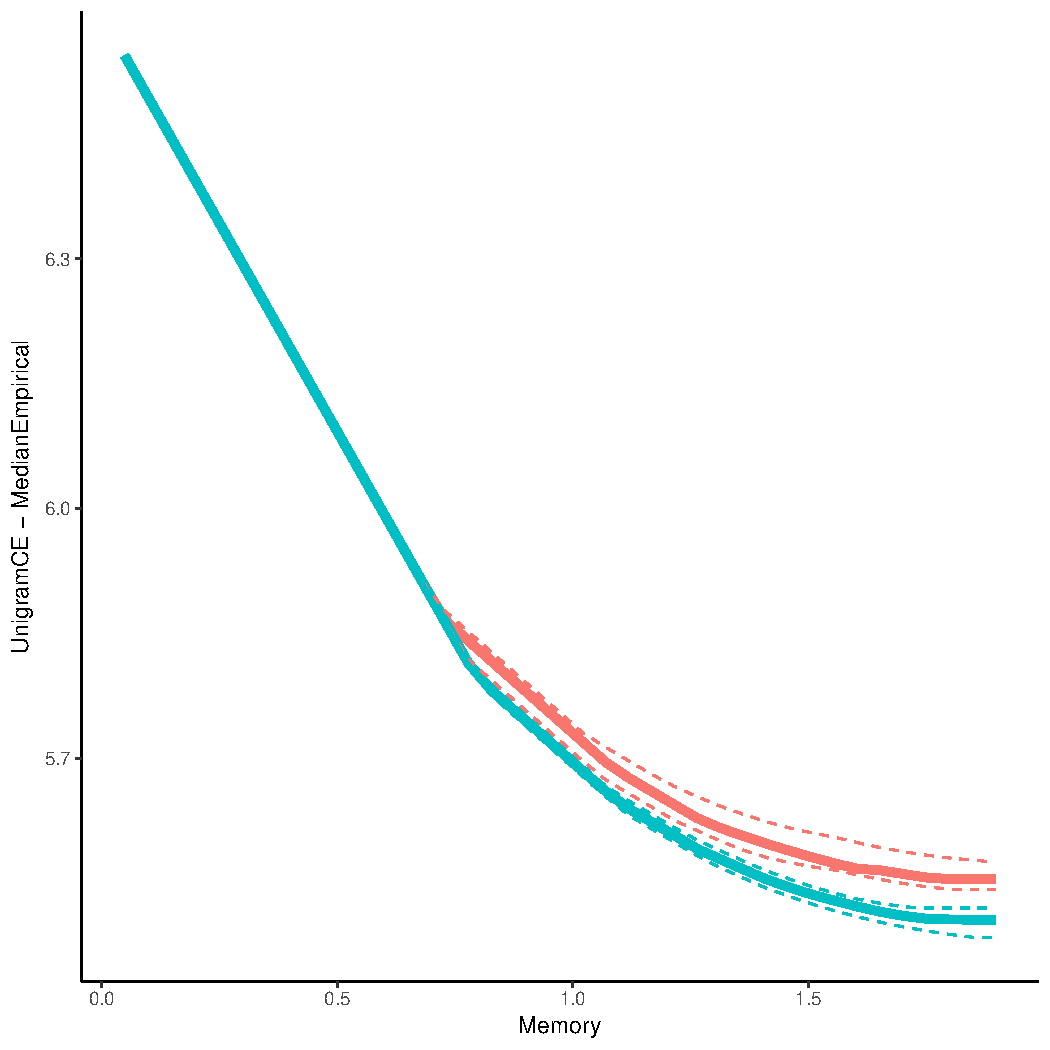
\includegraphics[width=0.1\textwidth]{neural/figures/German-listener-surprisal-memory-MEDIANS_onlyWordForms_boundedVocab_REAL.pdf} & 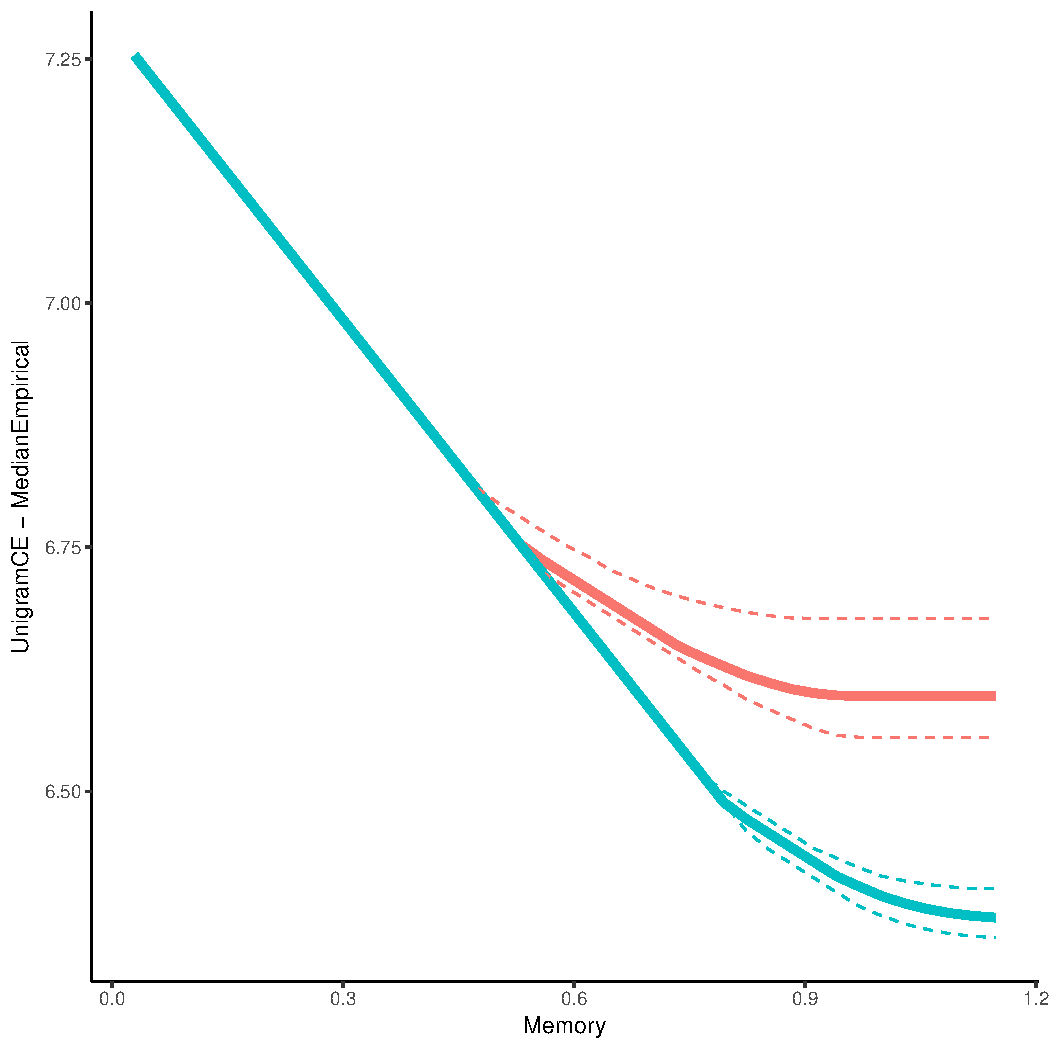
\includegraphics[width=0.1\textwidth]{neural/figures/Greek-listener-surprisal-memory-MEDIANS_onlyWordForms_boundedVocab_REAL.pdf} & 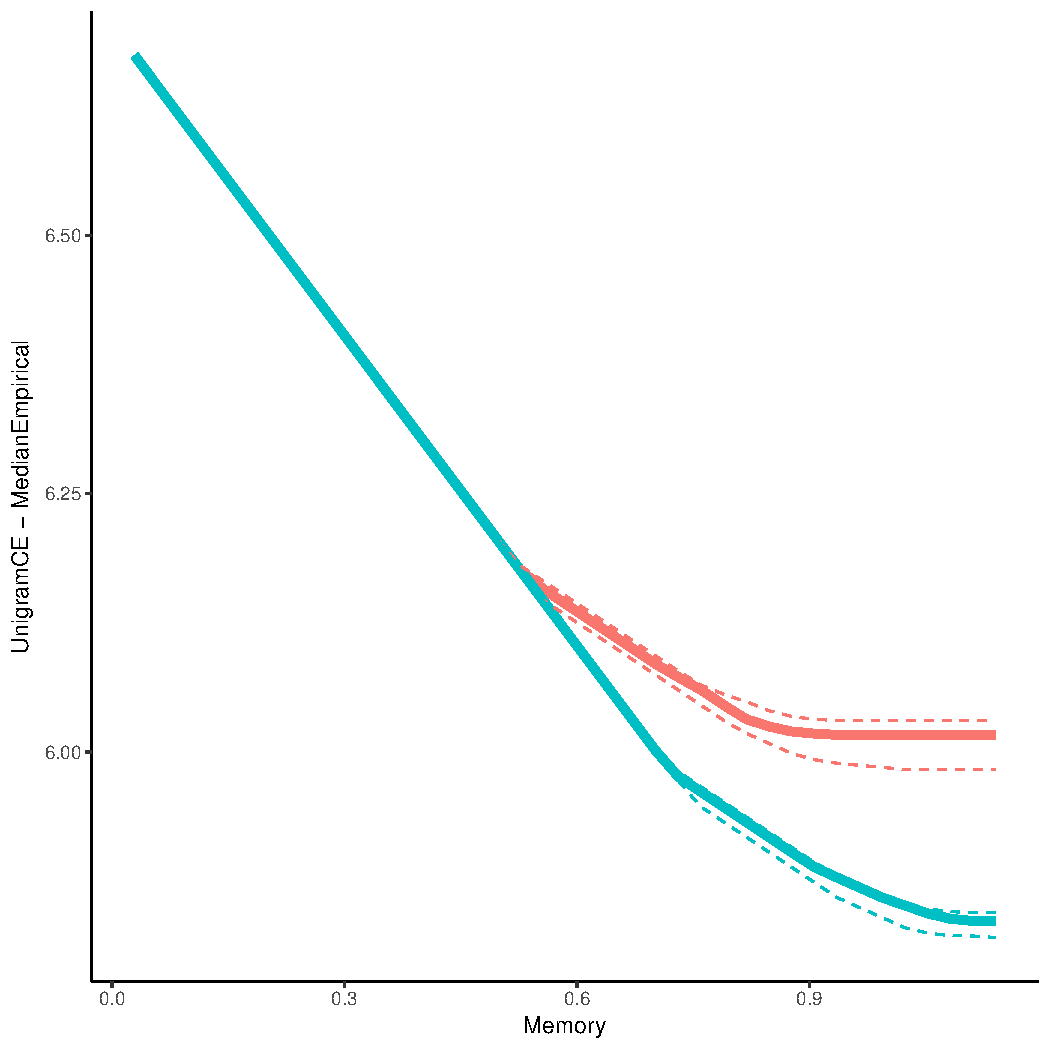
\includegraphics[width=0.1\textwidth]{neural/figures/Hebrew-listener-surprisal-memory-MEDIANS_onlyWordForms_boundedVocab_REAL.pdf} & 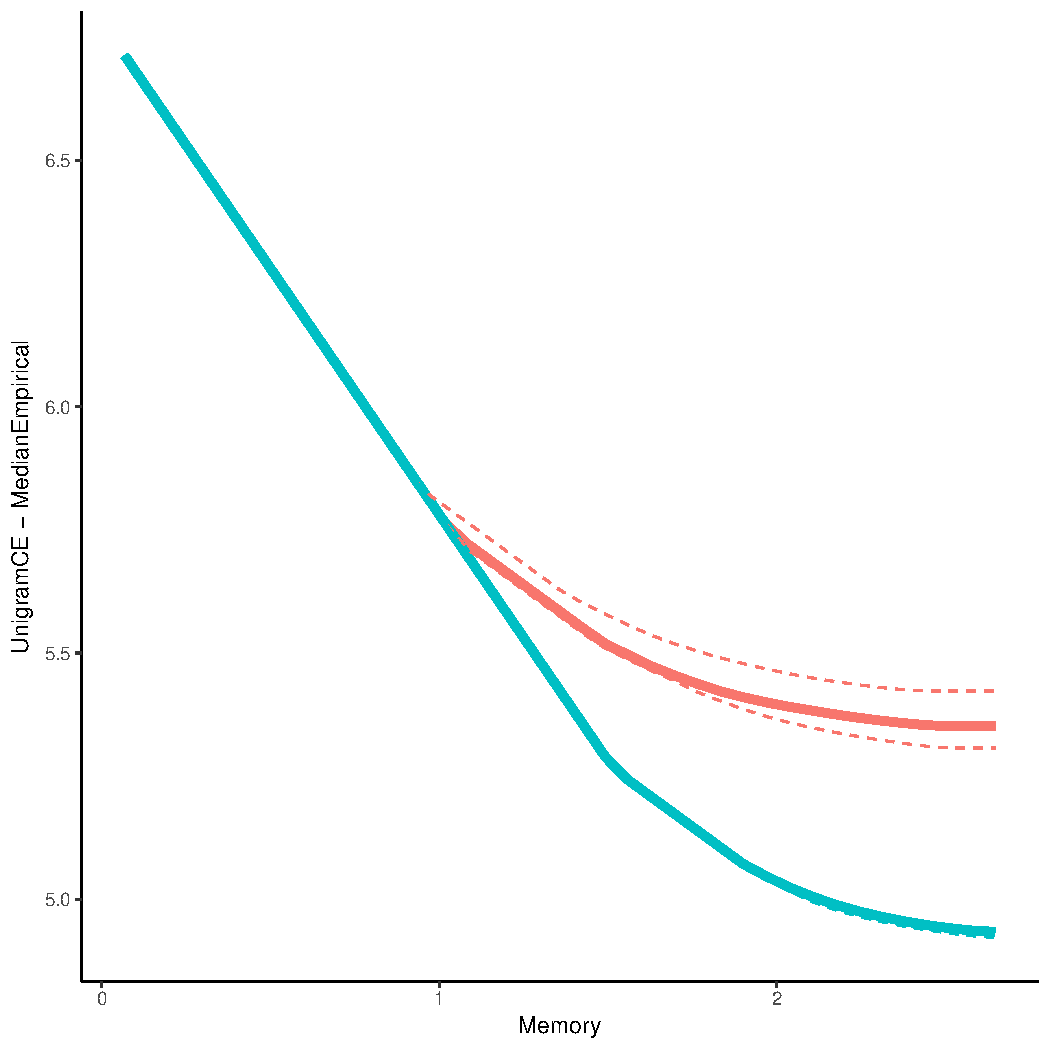
\includegraphics[width=0.1\textwidth]{neural/figures/Hindi-listener-surprisal-memory-MEDIANS_onlyWordForms_boundedVocab_REAL.pdf} & 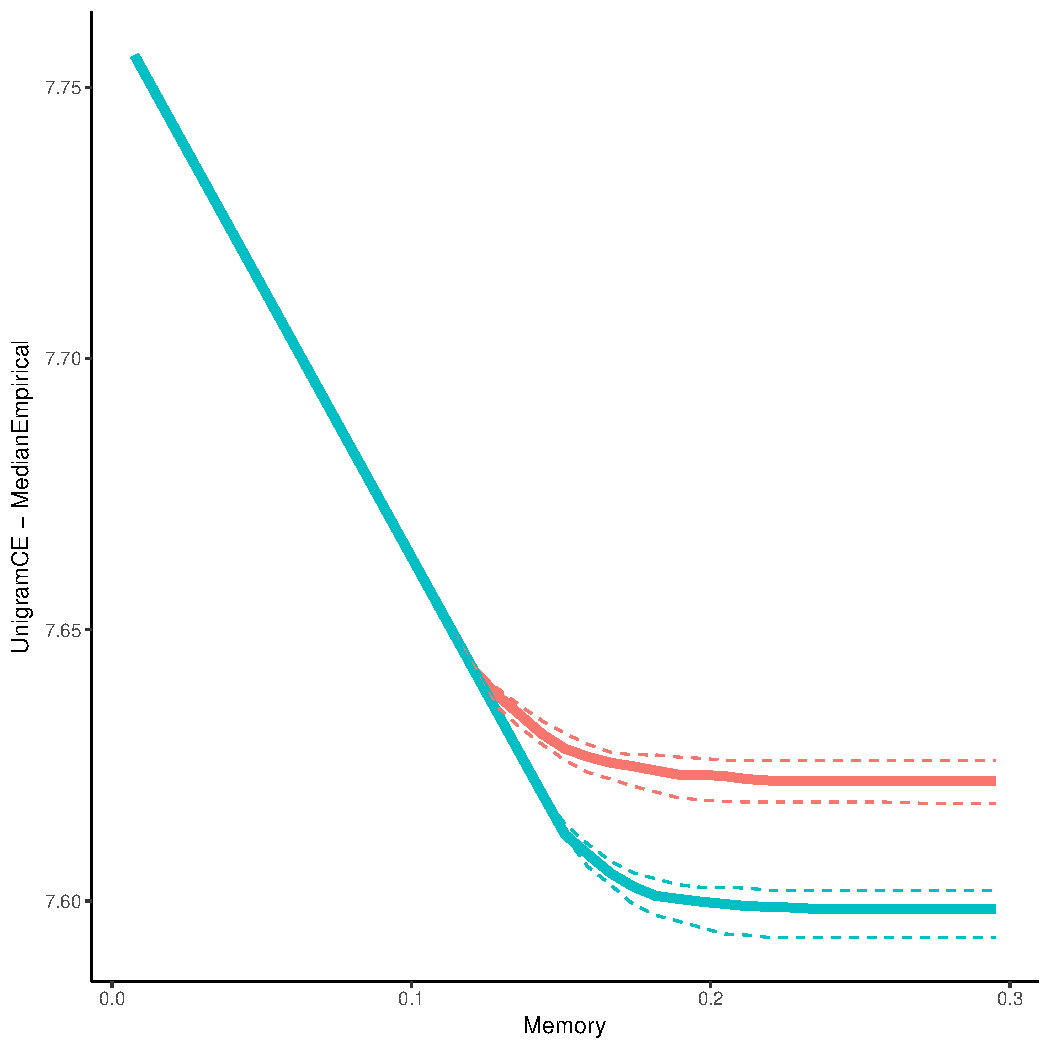
\includegraphics[width=0.1\textwidth]{neural/figures/Hungarian-listener-surprisal-memory-MEDIANS_onlyWordForms_boundedVocab_REAL.pdf}
 \\ 
Indonesian & Italian & Japanese & Kazakh & Korean & Kurmanji & Latvian & Maltese & Naija
 \\ 
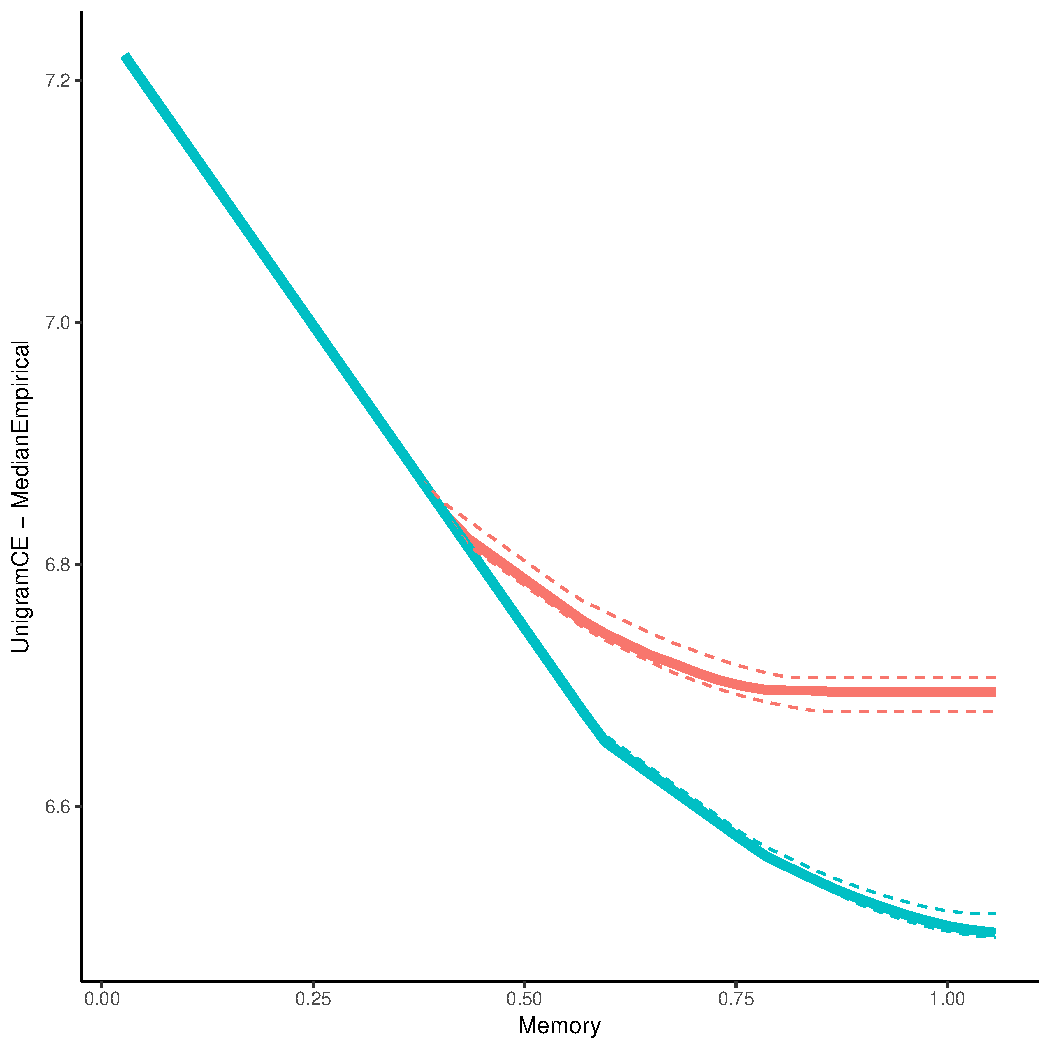
\includegraphics[width=0.1\textwidth]{neural/figures/Indonesian-listener-surprisal-memory-MEDIANS_onlyWordForms_boundedVocab_REAL.pdf} & 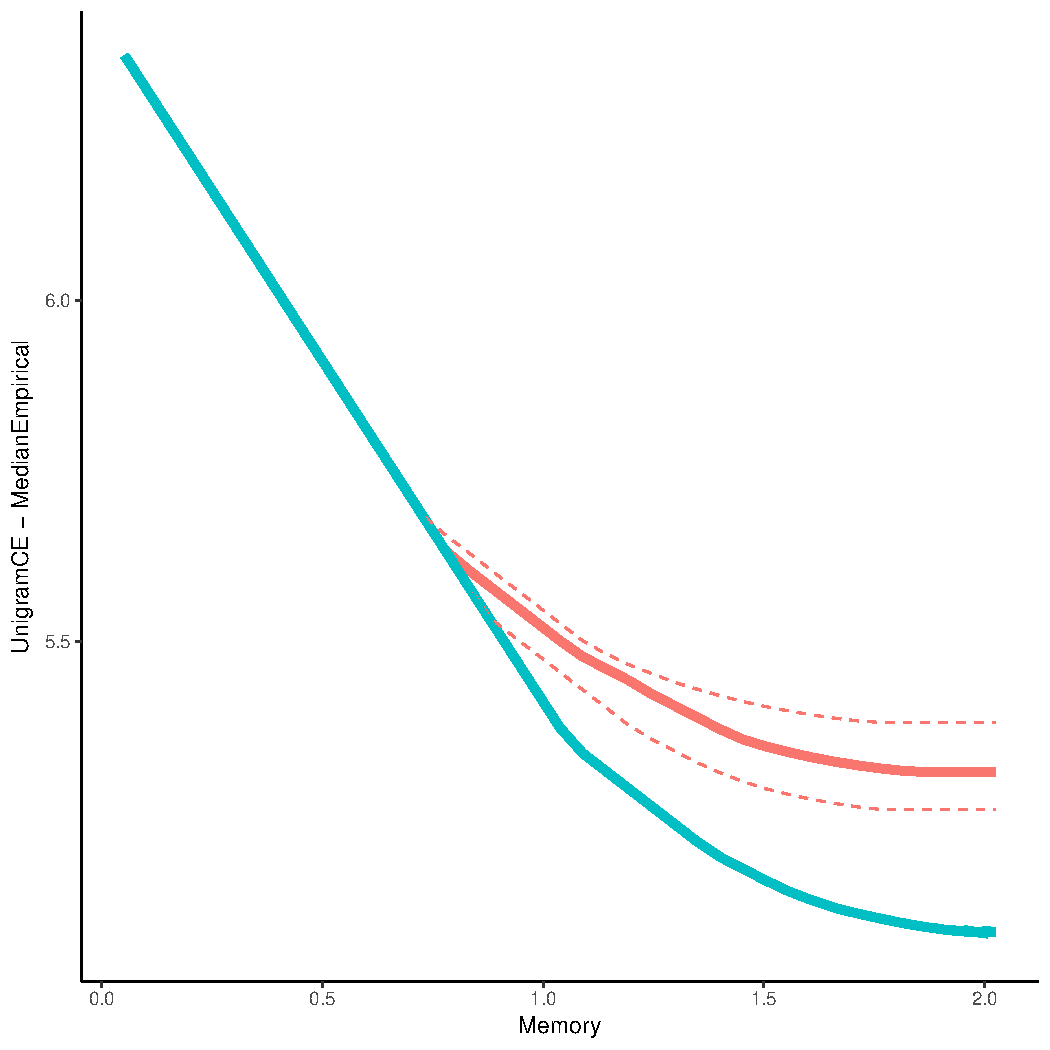
\includegraphics[width=0.1\textwidth]{neural/figures/Italian-listener-surprisal-memory-MEDIANS_onlyWordForms_boundedVocab_REAL.pdf} & 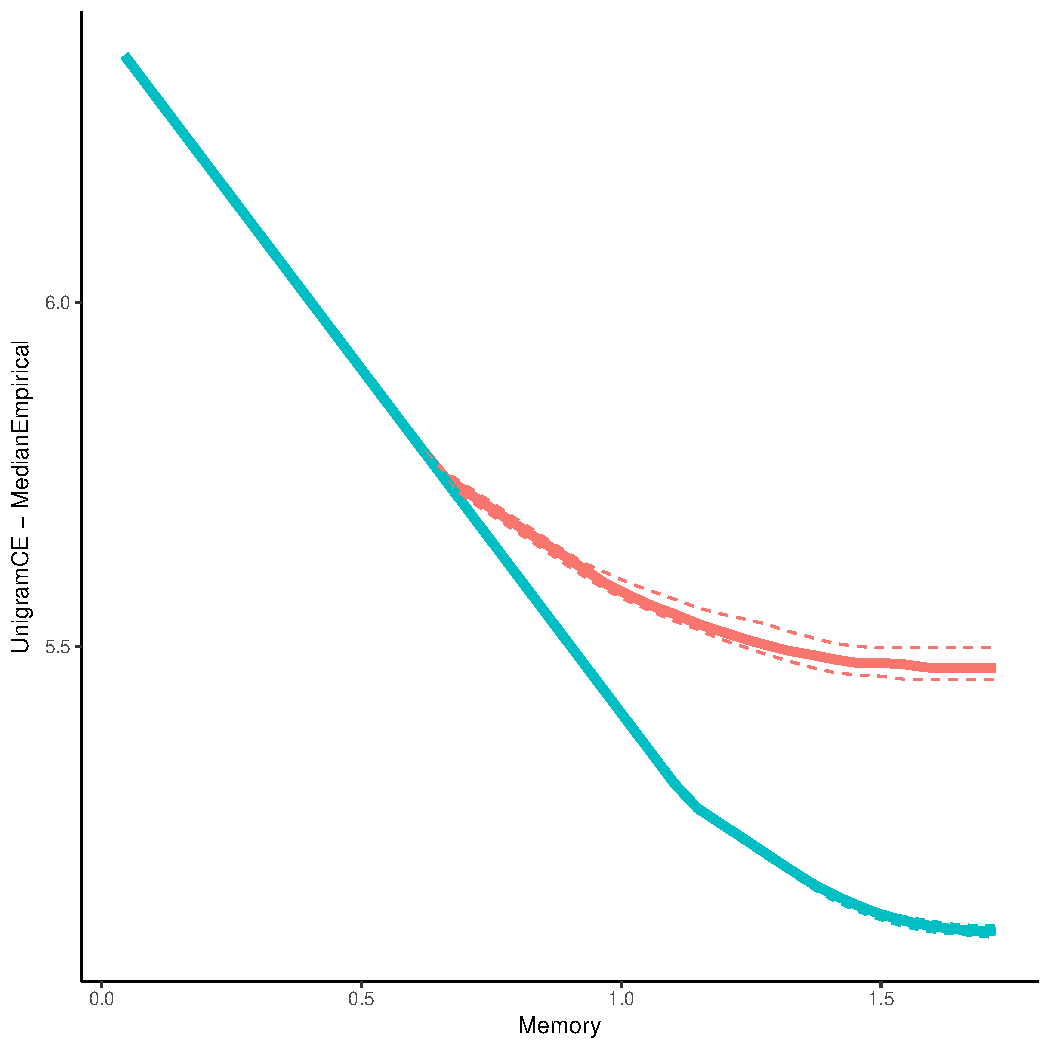
\includegraphics[width=0.1\textwidth]{neural/figures/Japanese-listener-surprisal-memory-MEDIANS_onlyWordForms_boundedVocab_REAL.pdf} & 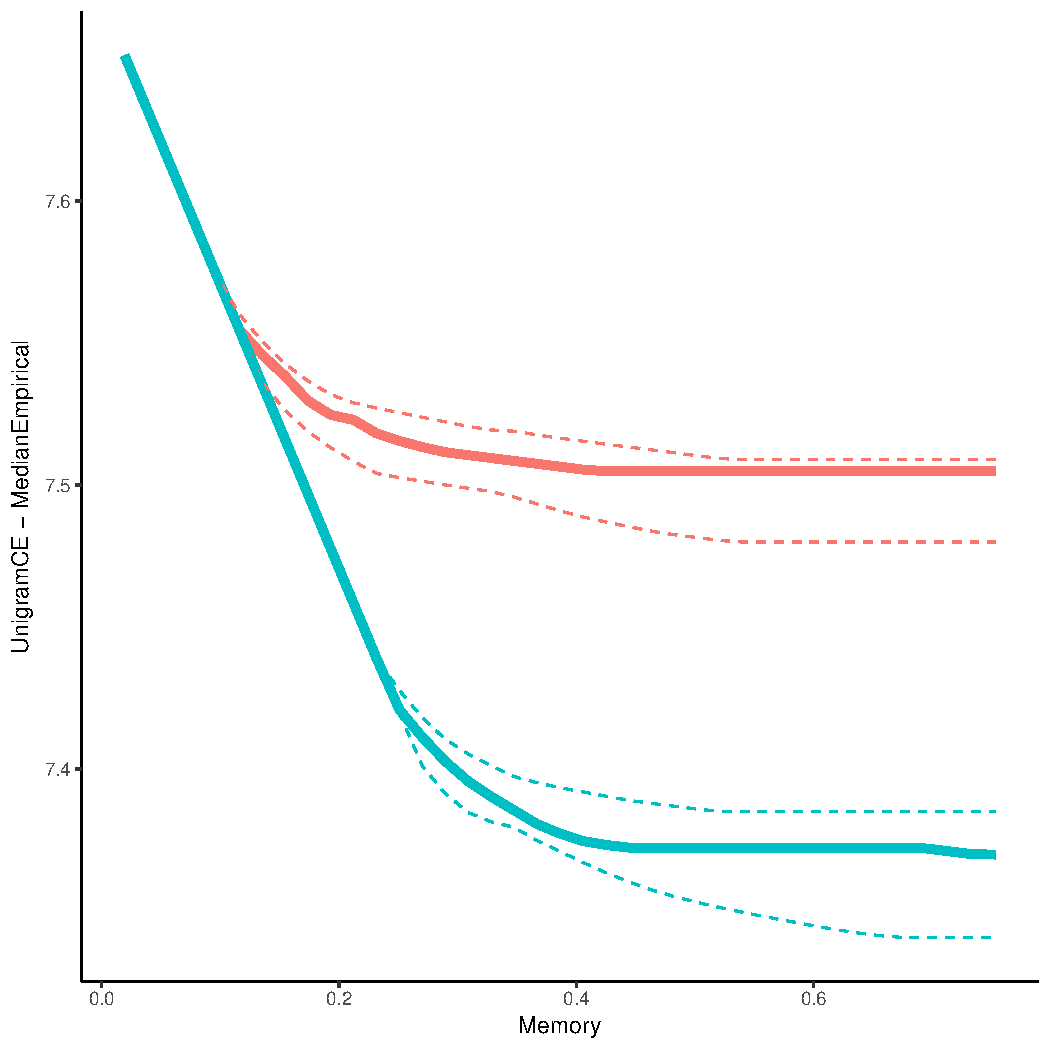
\includegraphics[width=0.1\textwidth]{neural/figures/Kazakh-Adap-listener-surprisal-memory-MEDIANS_onlyWordForms_boundedVocab_REAL.pdf} & 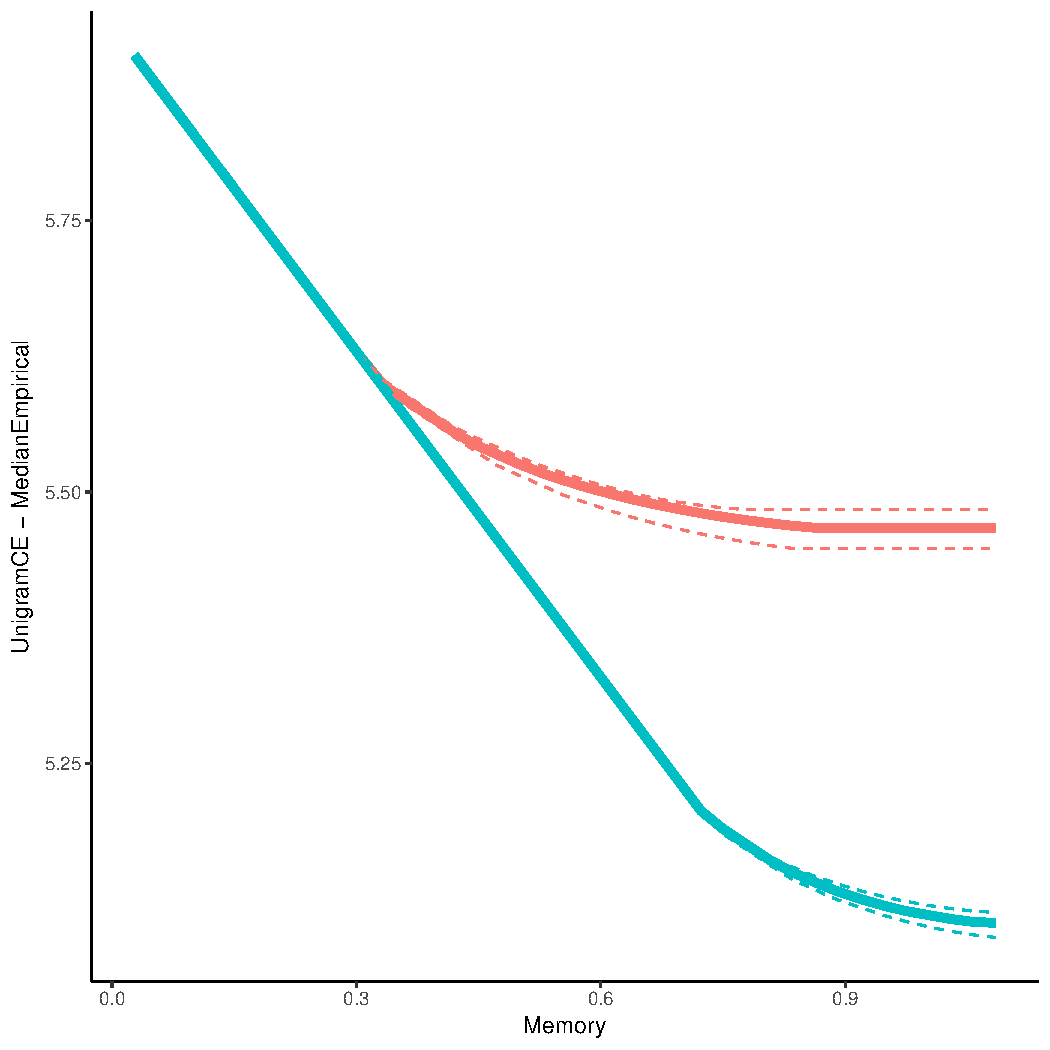
\includegraphics[width=0.1\textwidth]{neural/figures/Korean-listener-surprisal-memory-MEDIANS_onlyWordForms_boundedVocab_REAL.pdf} & 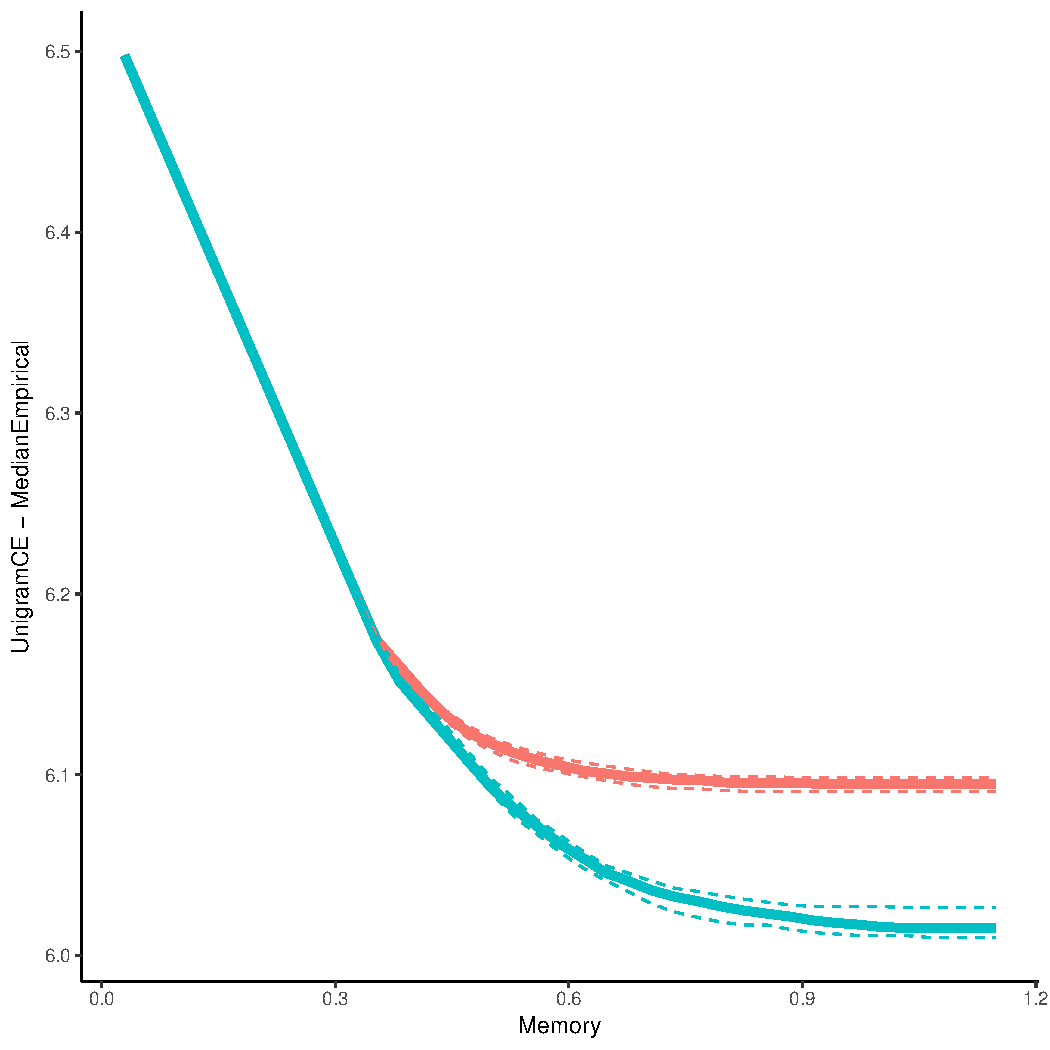
\includegraphics[width=0.1\textwidth]{neural/figures/Kurmanji-Adap-listener-surprisal-memory-MEDIANS_onlyWordForms_boundedVocab_REAL.pdf} & 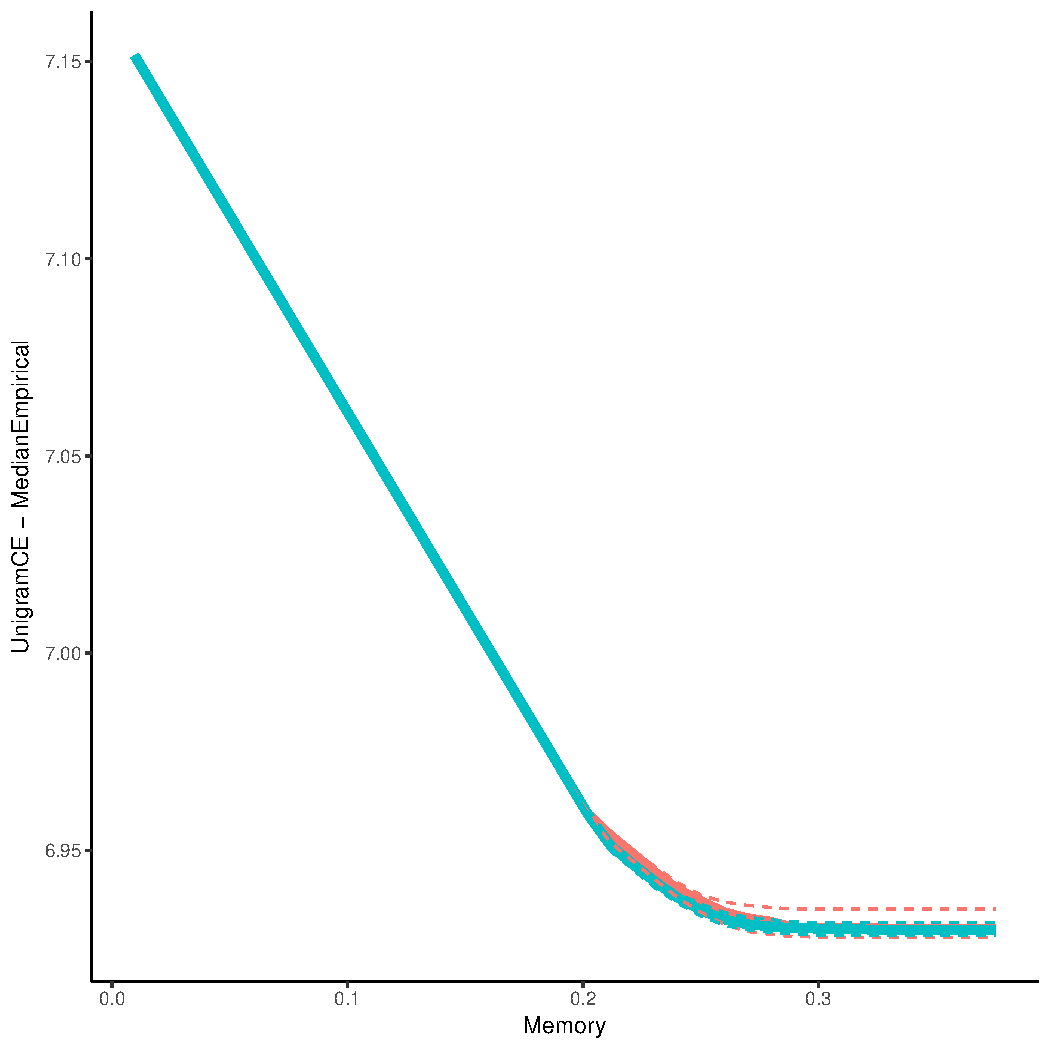
\includegraphics[width=0.1\textwidth]{neural/figures/Latvian-listener-surprisal-memory-MEDIANS_onlyWordForms_boundedVocab_REAL.pdf} & 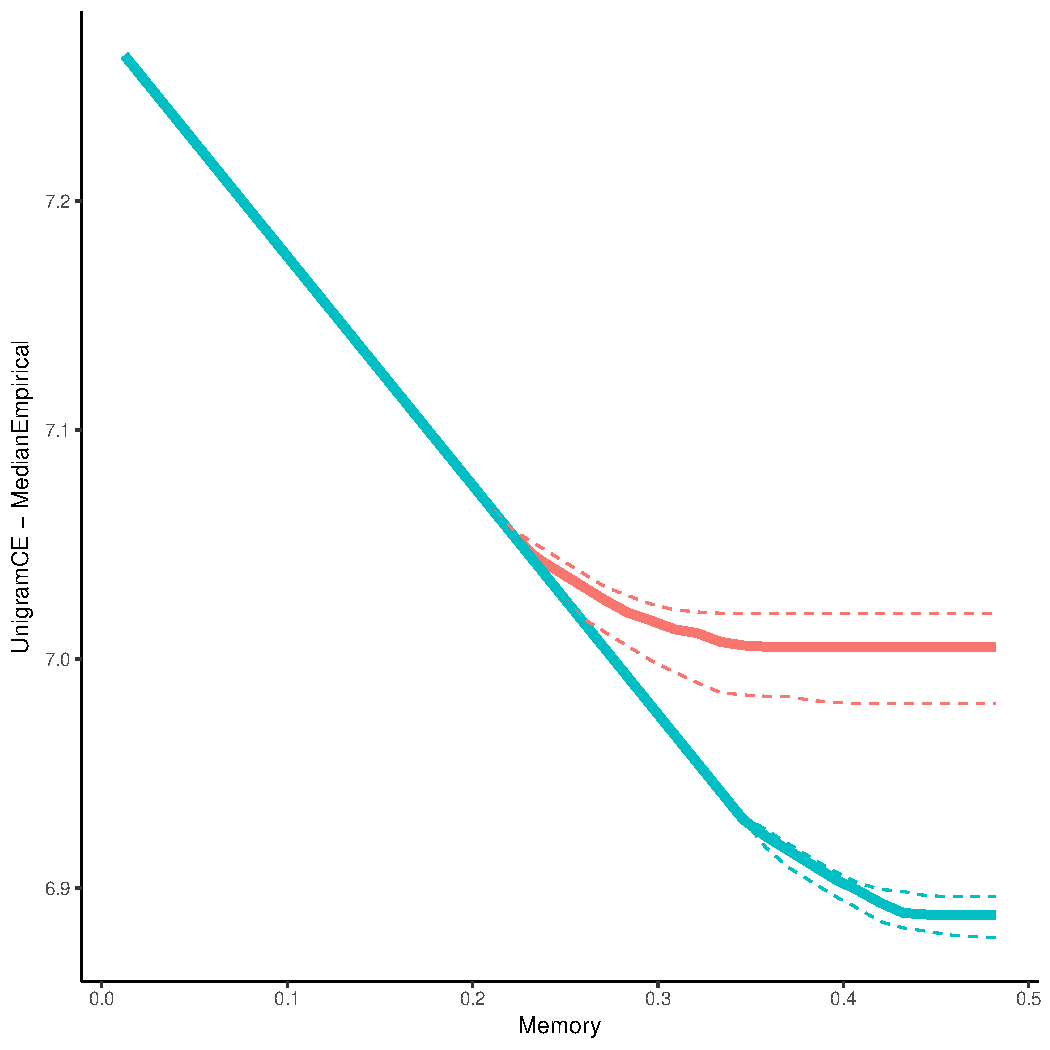
\includegraphics[width=0.1\textwidth]{neural/figures/Maltese-listener-surprisal-memory-MEDIANS_onlyWordForms_boundedVocab_REAL.pdf} & 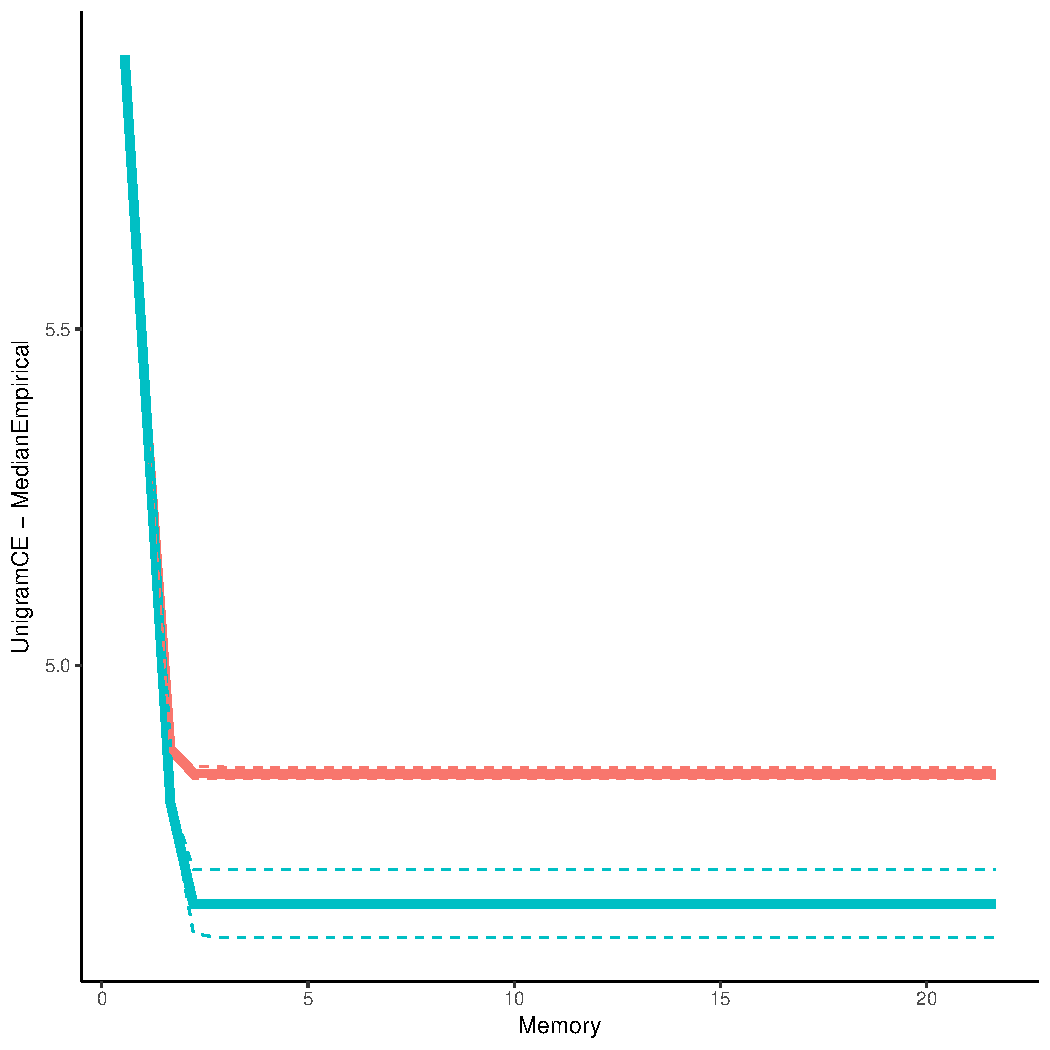
\includegraphics[width=0.1\textwidth]{neural/figures/Naija-Adap-listener-surprisal-memory-MEDIANS_onlyWordForms_boundedVocab_REAL.pdf}
 \\ 
North Sami & Norwegian & Persian & Polish & Portuguese & Romanian & Russian & Serbian & Slovak
 \\ 
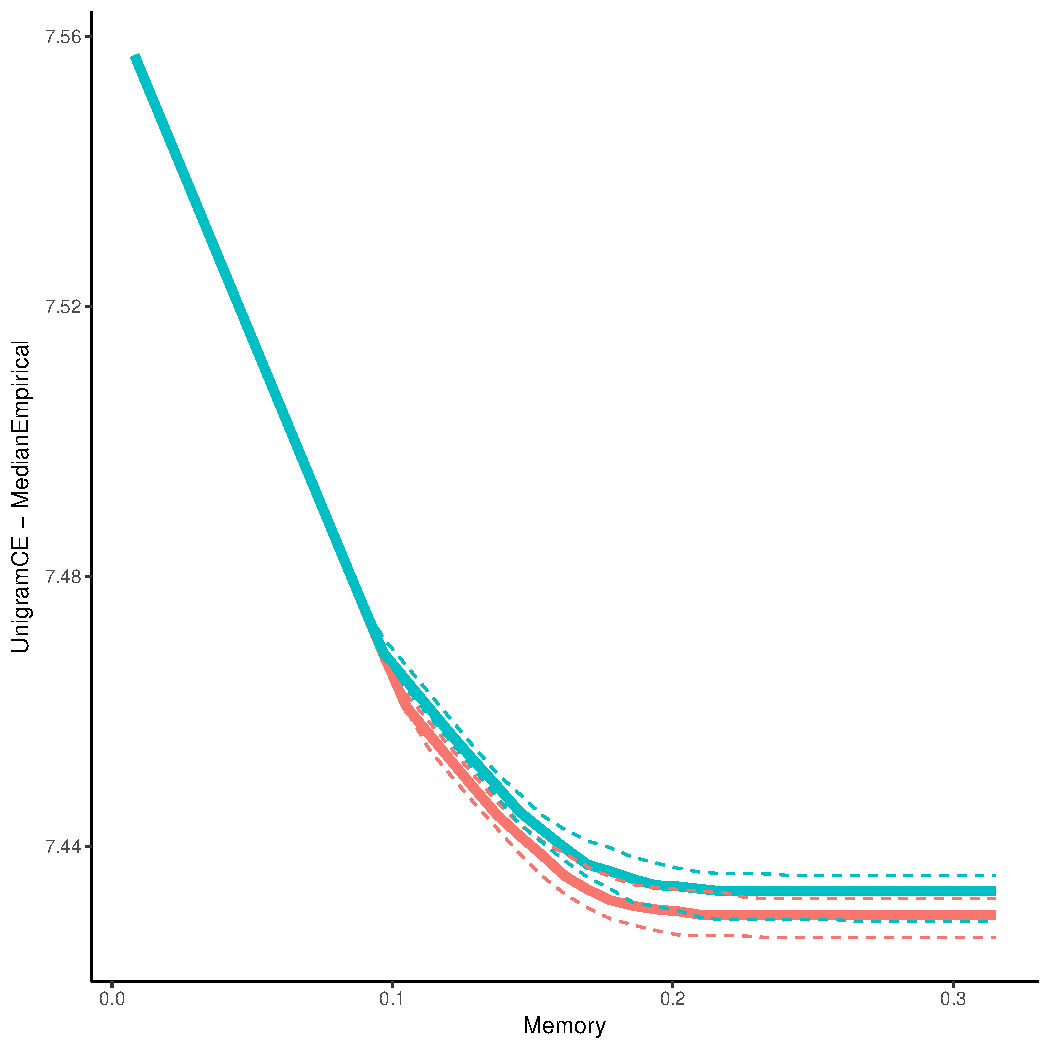
\includegraphics[width=0.1\textwidth]{neural/figures/North_Sami-listener-surprisal-memory-MEDIANS_onlyWordForms_boundedVocab_REAL.pdf} & 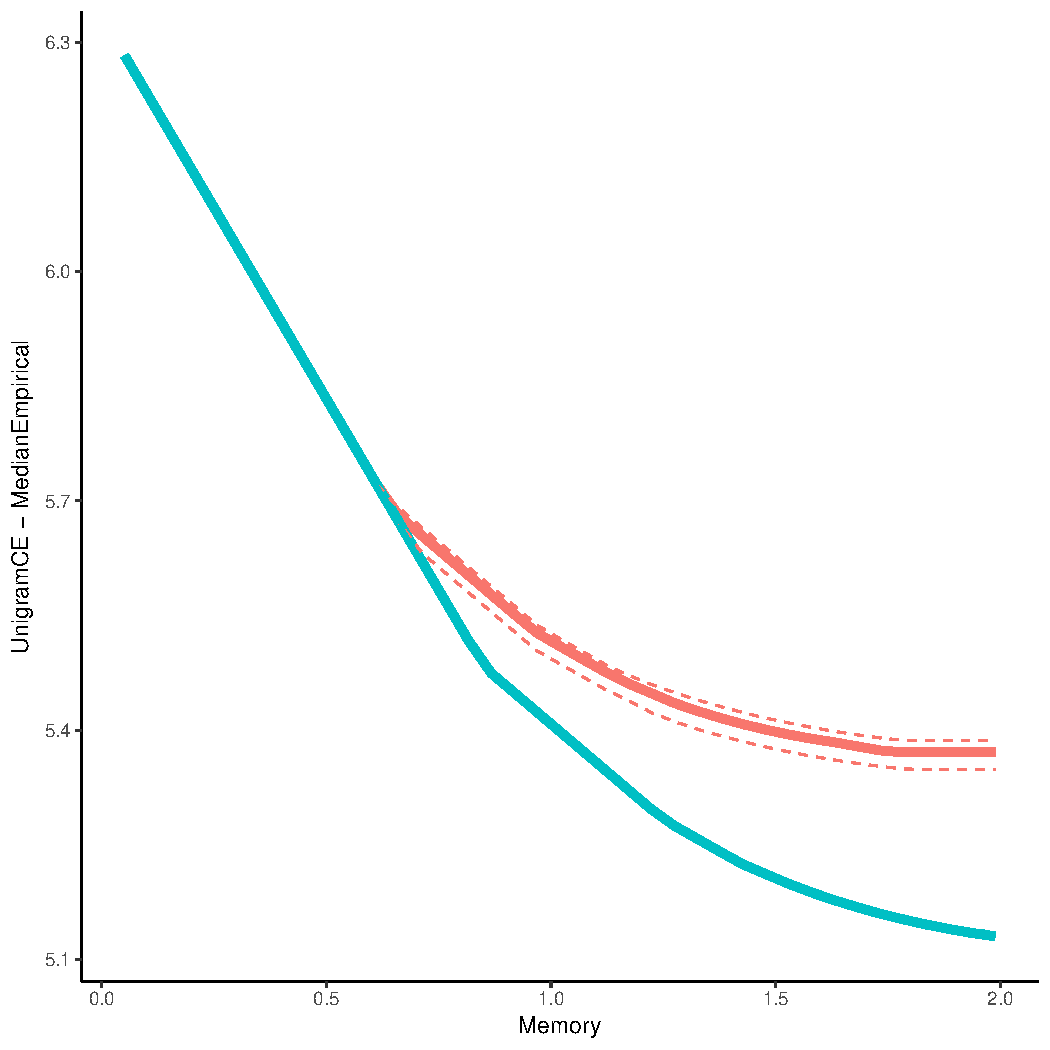
\includegraphics[width=0.1\textwidth]{neural/figures/Norwegian-listener-surprisal-memory-MEDIANS_onlyWordForms_boundedVocab_REAL.pdf} & 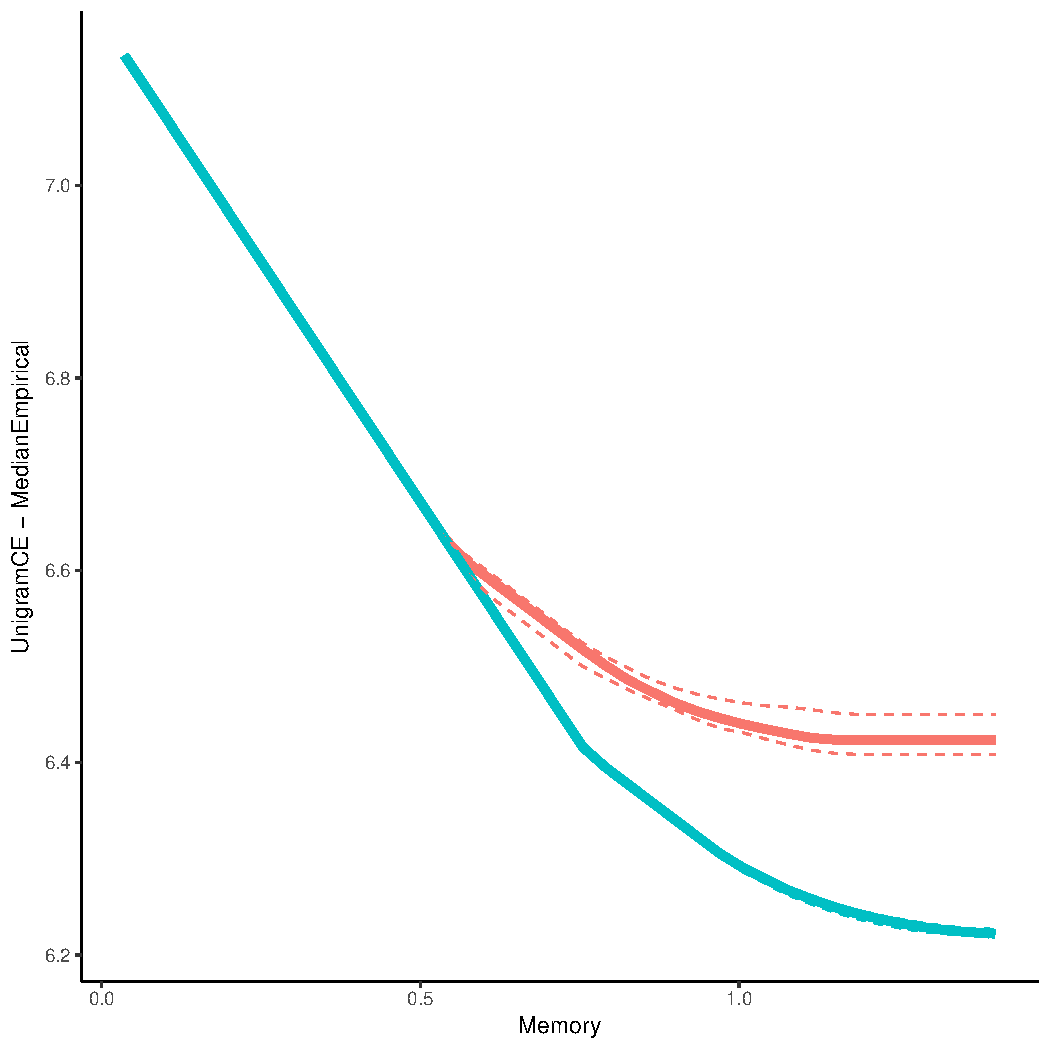
\includegraphics[width=0.1\textwidth]{neural/figures/Persian-listener-surprisal-memory-MEDIANS_onlyWordForms_boundedVocab_REAL.pdf} & 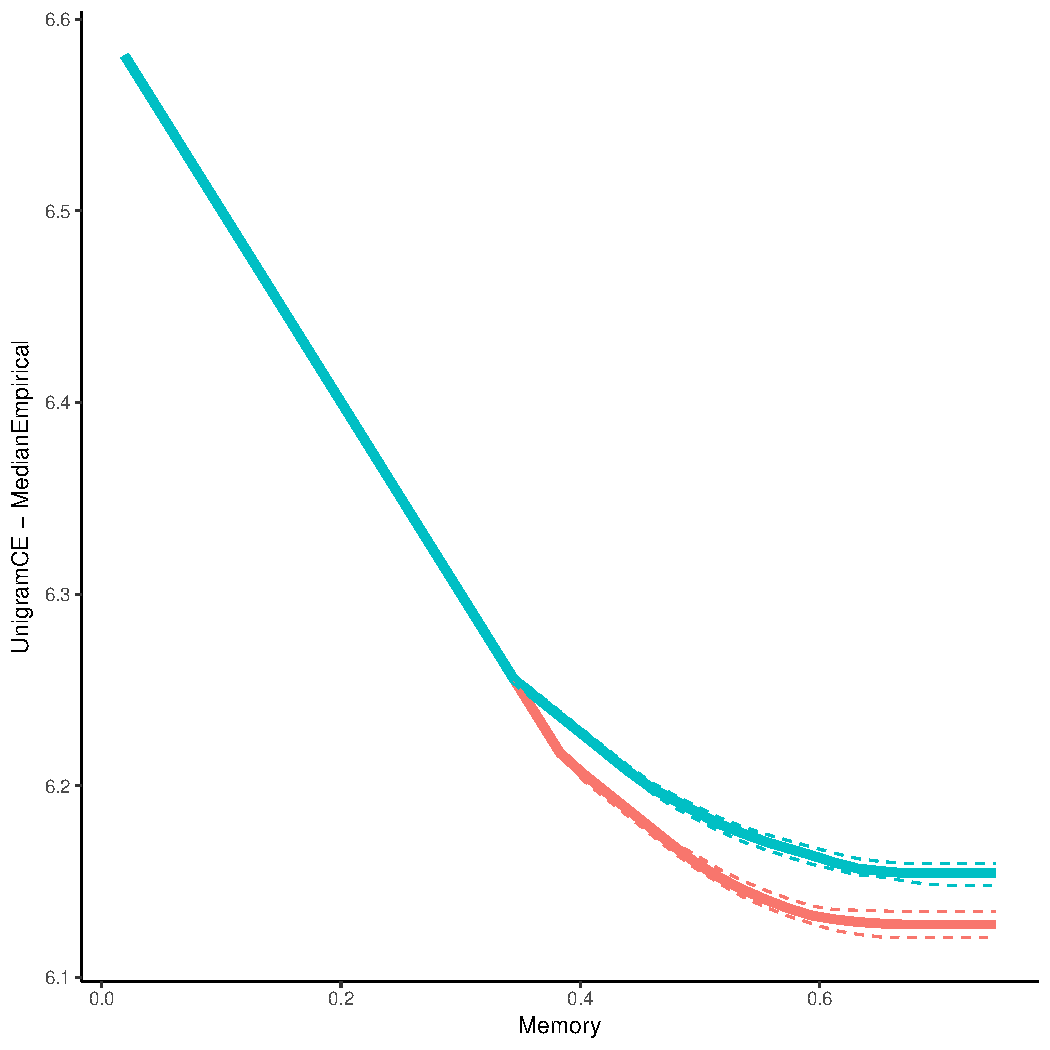
\includegraphics[width=0.1\textwidth]{neural/figures/Polish-listener-surprisal-memory-MEDIANS_onlyWordForms_boundedVocab_REAL.pdf} & 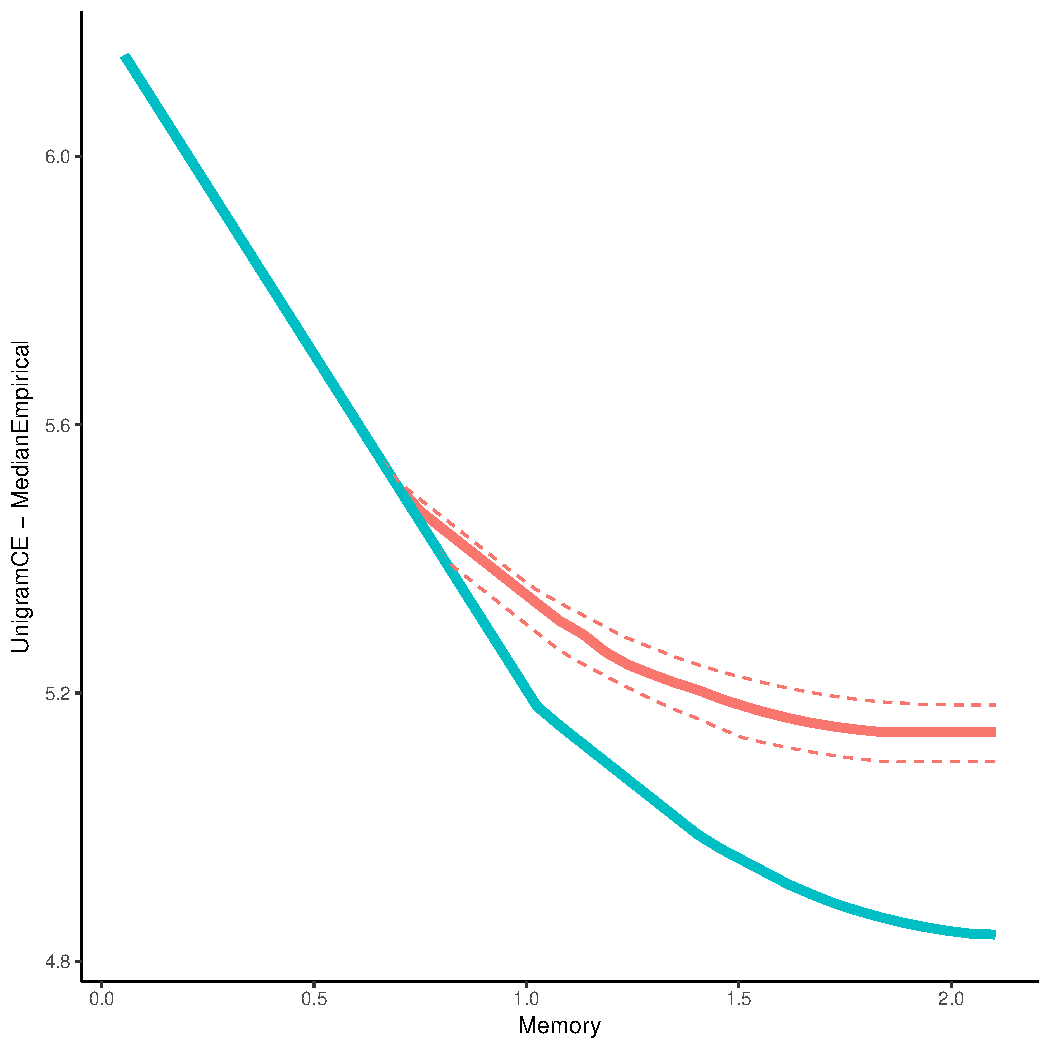
\includegraphics[width=0.1\textwidth]{neural/figures/Portuguese-listener-surprisal-memory-MEDIANS_onlyWordForms_boundedVocab_REAL.pdf} & 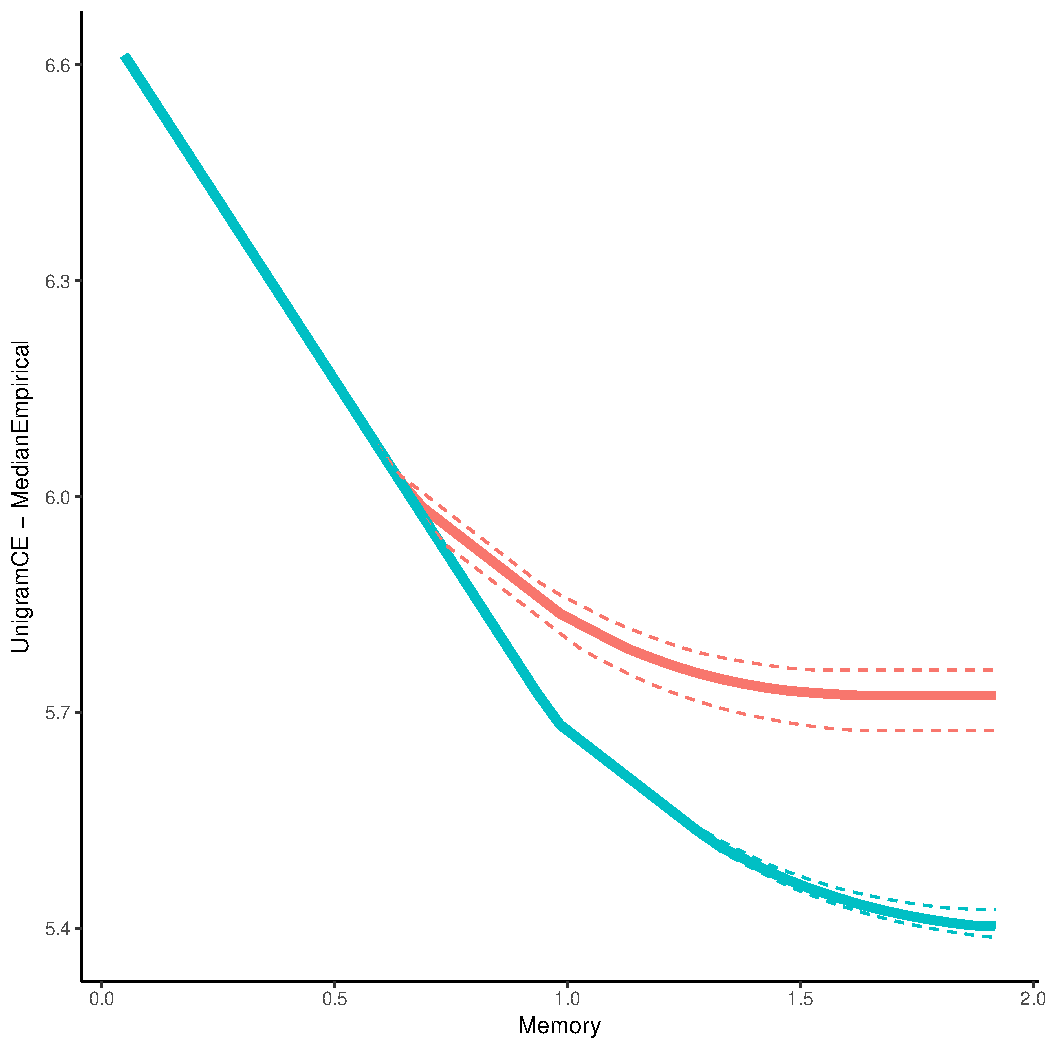
\includegraphics[width=0.1\textwidth]{neural/figures/Romanian-listener-surprisal-memory-MEDIANS_onlyWordForms_boundedVocab_REAL.pdf} & 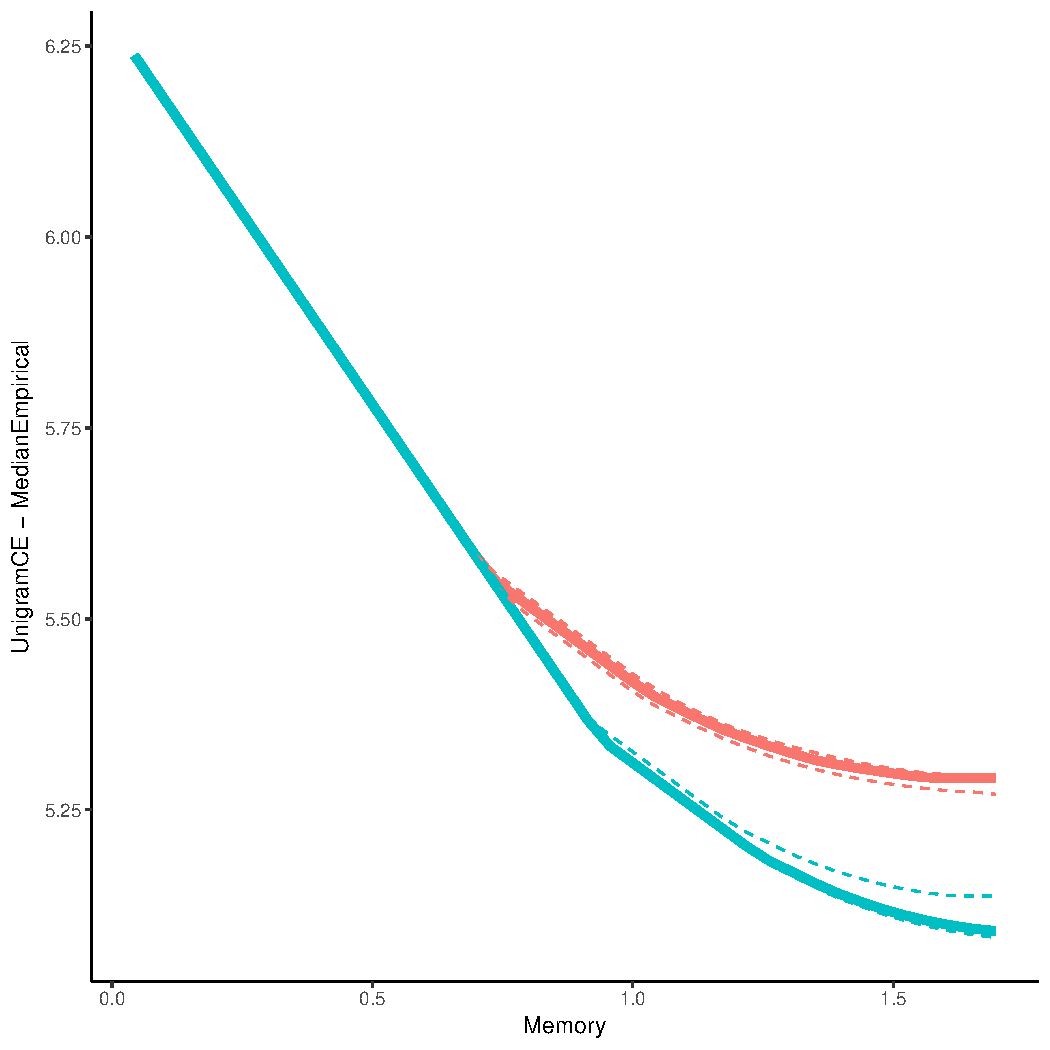
\includegraphics[width=0.1\textwidth]{neural/figures/Russian-listener-surprisal-memory-MEDIANS_onlyWordForms_boundedVocab_REAL.pdf} & 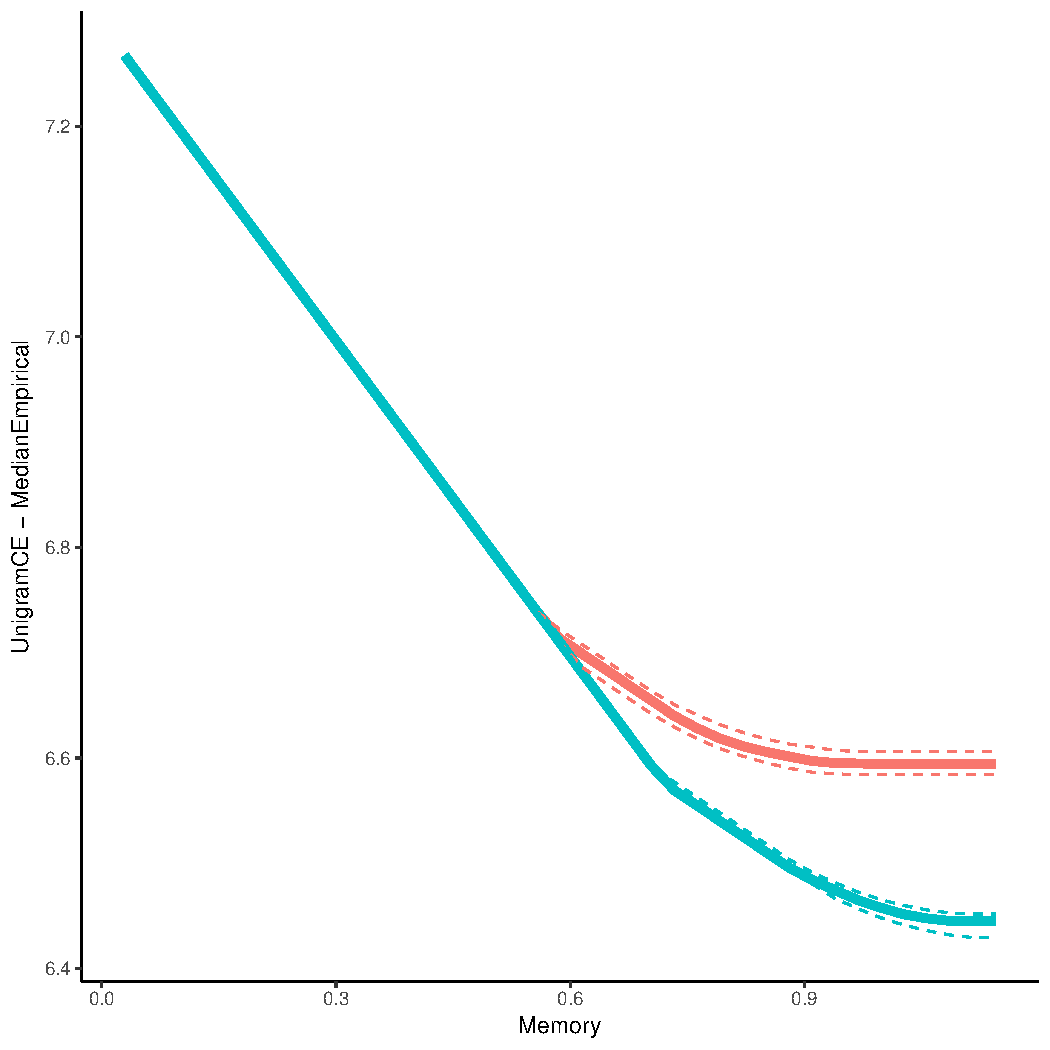
\includegraphics[width=0.1\textwidth]{neural/figures/Serbian-listener-surprisal-memory-MEDIANS_onlyWordForms_boundedVocab_REAL.pdf} & 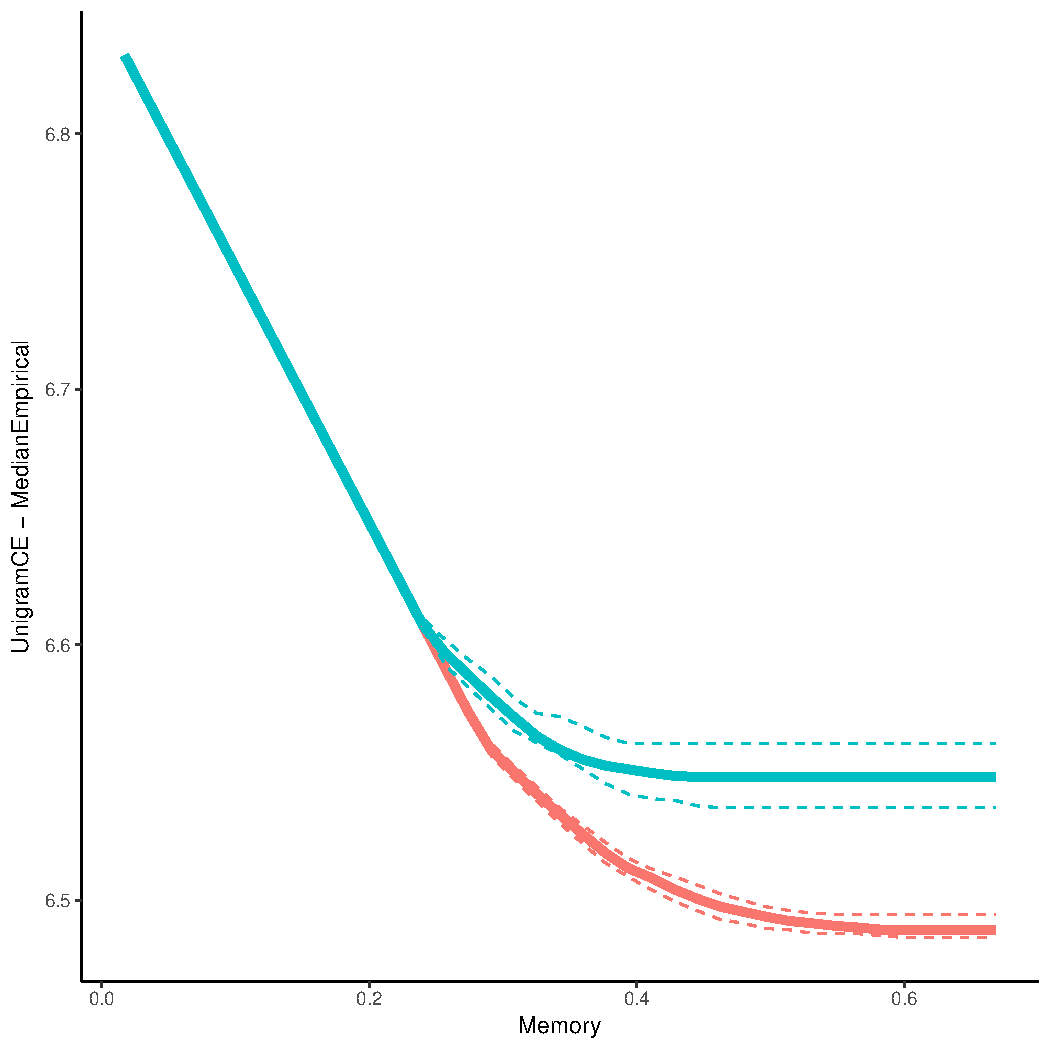
\includegraphics[width=0.1\textwidth]{neural/figures/Slovak-listener-surprisal-memory-MEDIANS_onlyWordForms_boundedVocab_REAL.pdf}
 \\ 
Slovenian & Spanish & Swedish & Thai & Turkish & Ukrainian & Urdu & Uyghur & Vietnamese
 \\ 
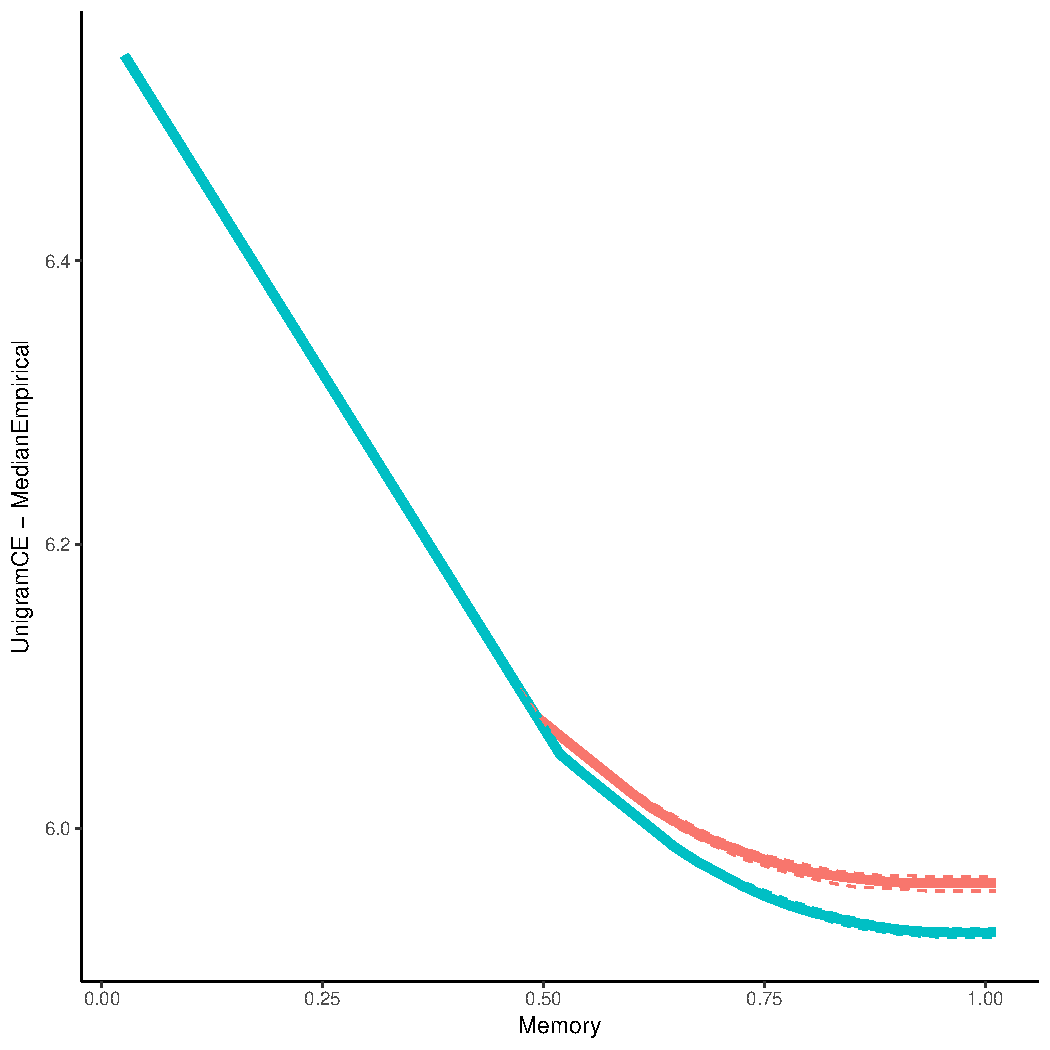
\includegraphics[width=0.1\textwidth]{neural/figures/Slovenian-listener-surprisal-memory-MEDIANS_onlyWordForms_boundedVocab_REAL.pdf} & 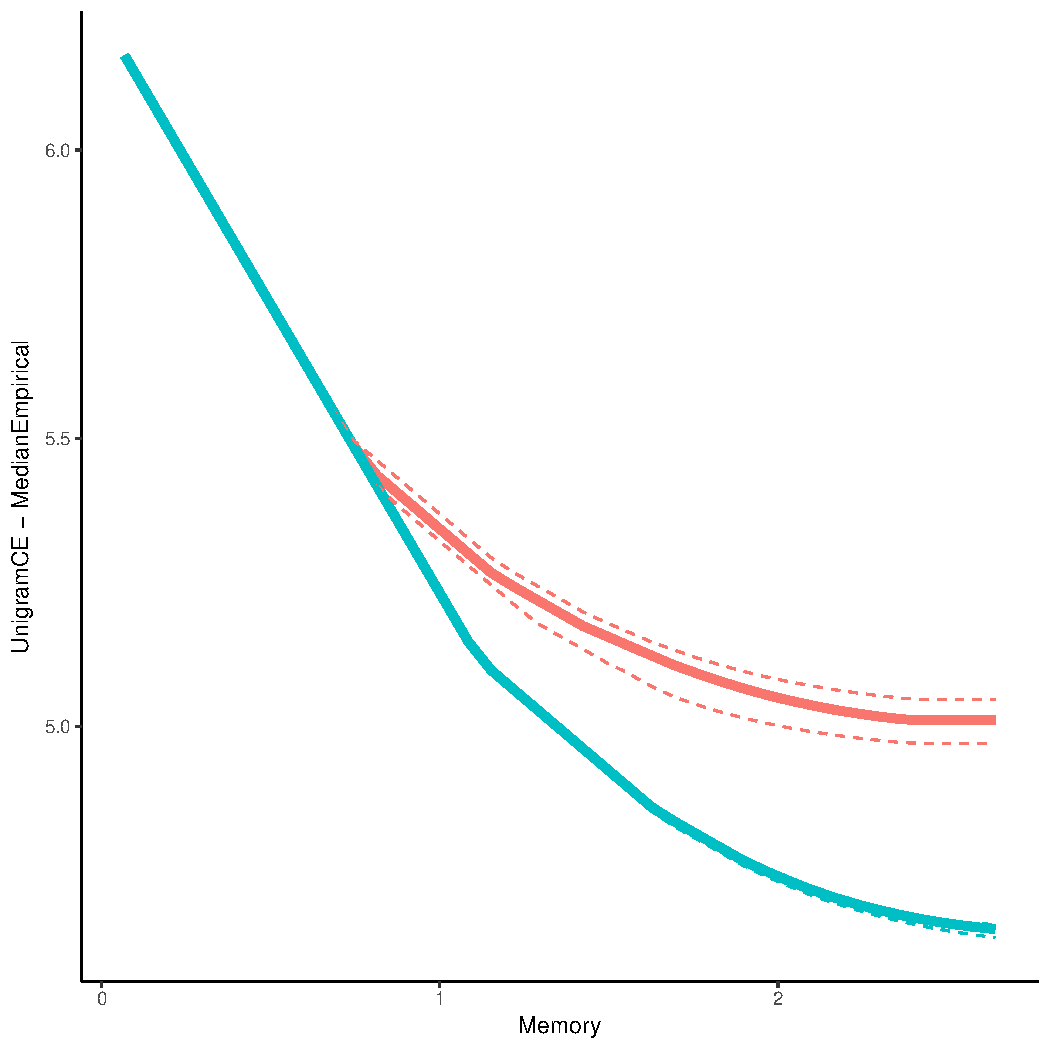
\includegraphics[width=0.1\textwidth]{neural/figures/Spanish-listener-surprisal-memory-MEDIANS_onlyWordForms_boundedVocab_REAL.pdf} & 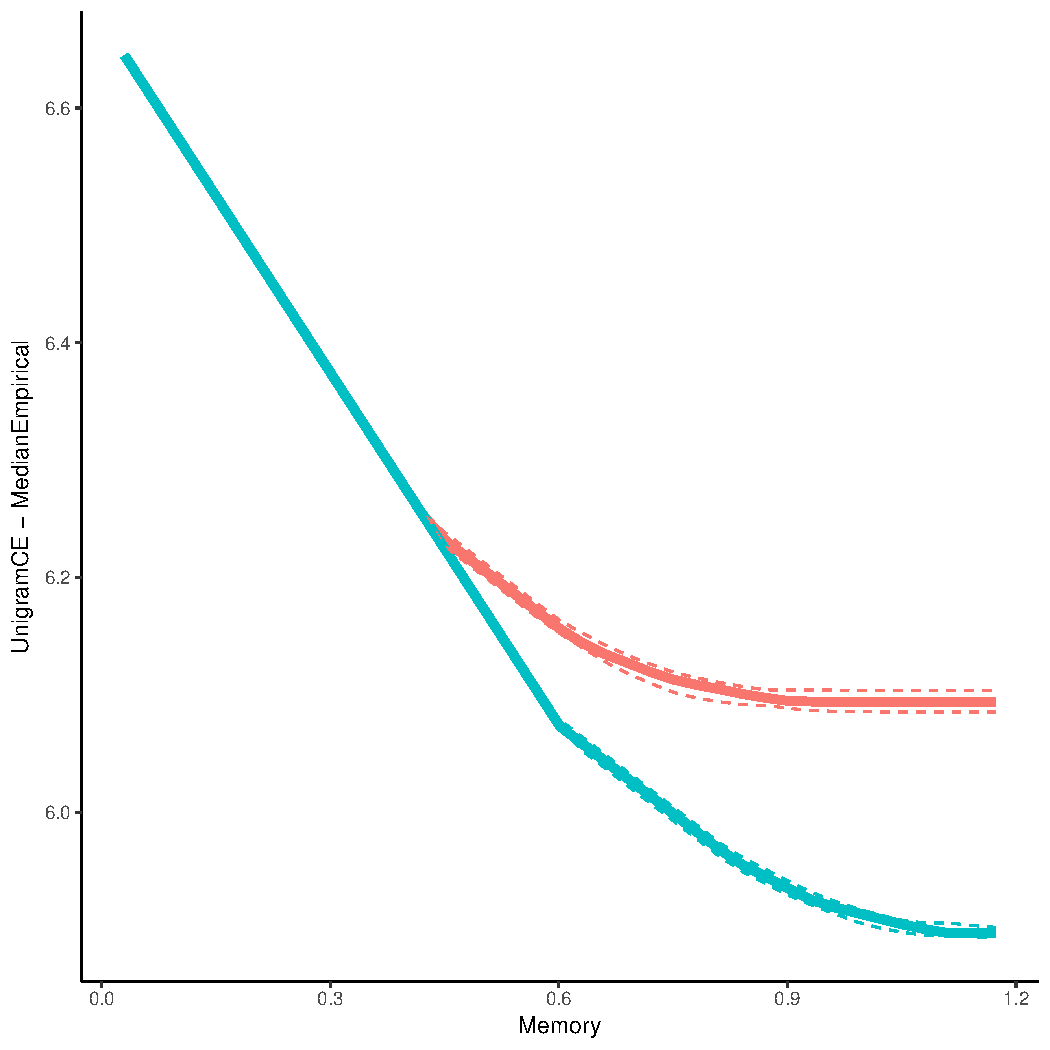
\includegraphics[width=0.1\textwidth]{neural/figures/Swedish-listener-surprisal-memory-MEDIANS_onlyWordForms_boundedVocab_REAL.pdf} & 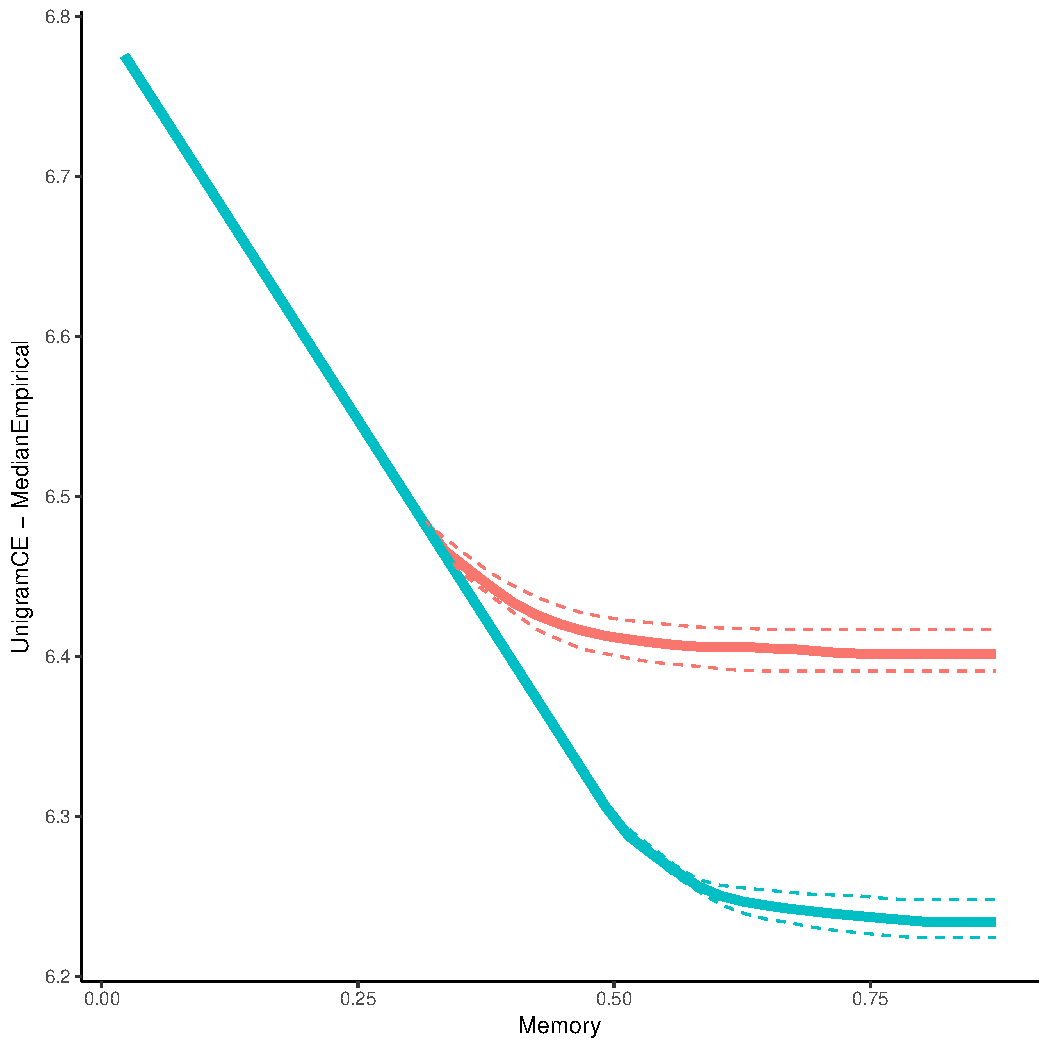
\includegraphics[width=0.1\textwidth]{neural/figures/Thai-Adap-listener-surprisal-memory-MEDIANS_onlyWordForms_boundedVocab_REAL.pdf} & 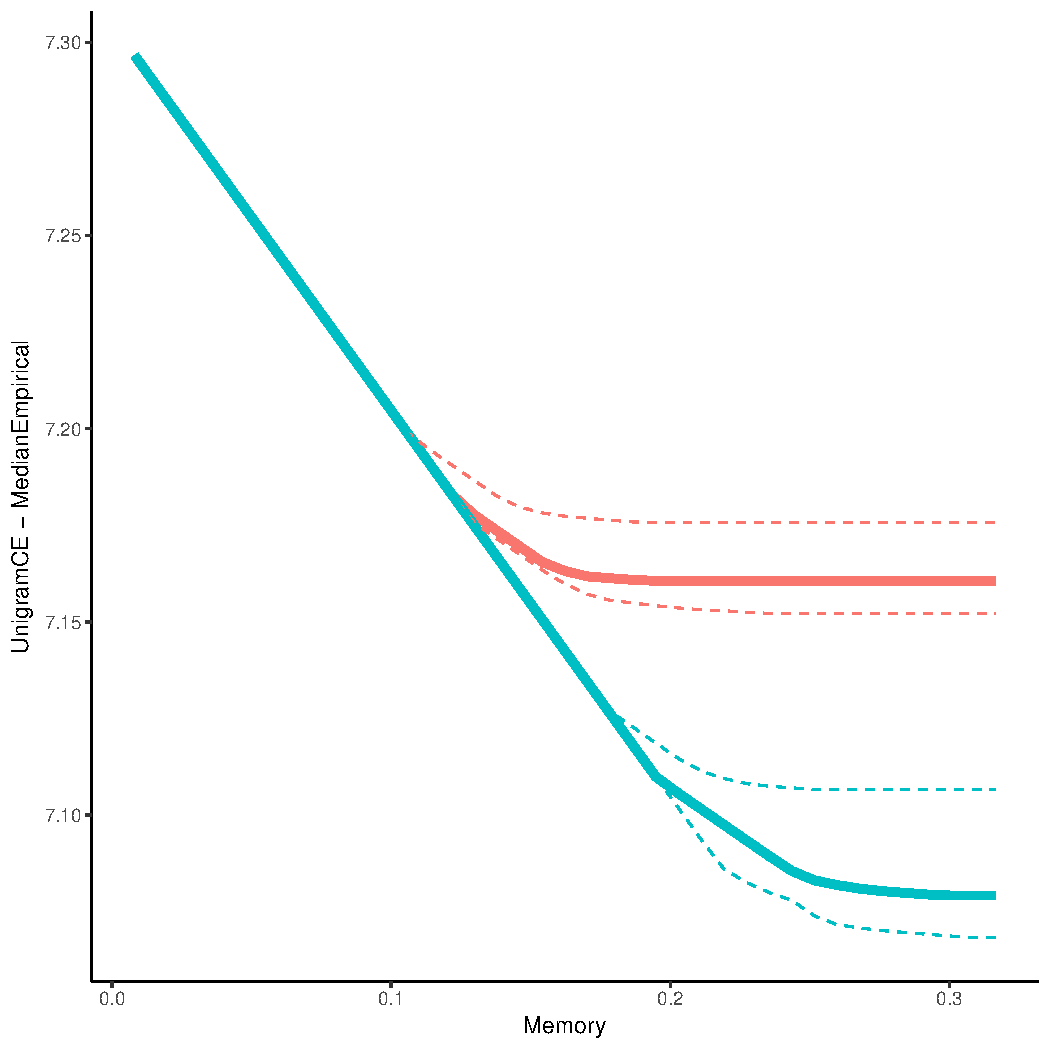
\includegraphics[width=0.1\textwidth]{neural/figures/Turkish-listener-surprisal-memory-MEDIANS_onlyWordForms_boundedVocab_REAL.pdf} & \includegraphics[width=0.1\textwidth]{neural/figures/Ukrainian-listener-surprisal-memory-MEDIANS_onlyWordForms_boundedVocab_REAL.pdf} & \includegraphics[width=0.1\textwidth]{neural/figures/Urdu-listener-surprisal-memory-MEDIANS_onlyWordForms_boundedVocab_REAL.pdf} & \includegraphics[width=0.1\textwidth]{neural/figures/Uyghur-Adap-listener-surprisal-memory-MEDIANS_onlyWordForms_boundedVocab_REAL.pdf} & \includegraphics[width=0.1\textwidth]{neural/figures/Vietnamese-listener-surprisal-memory-MEDIANS_onlyWordForms_boundedVocab_REAL.pdf}
 \\ 

\end{longtable}
\end{table}


\end{document}
